\documentclass[12pt]{article}
\usepackage[utf8]{inputenc}
\usepackage[T1]{fontenc}
\usepackage{graphicx}
\usepackage{longtable}
\usepackage{wrapfig}
\usepackage{rotating}
\usepackage[normalem]{ulem}
\usepackage{amsmath}
\usepackage{amssymb}
\usepackage{capt-of}
\usepackage{hyperref}
\usepackage[danish, ]{babel}
\usepackage[margin=2.5cm]{geometry}
\usepackage{lmodern}
\usepackage[style=verbose-ibid,backend=bibtex]{biblatex}
\usepackage{csquotes}
\usepackage{comment}
\usepackage{float}
\usepackage{parskip}
\usepackage{fancyhdr}
\usepackage{setspace}
\usepackage{minted}
\usepackage{mdframed}
\usepackage{xcolor}
\usepackage[bottom]{footmisc}
\usepackage{booktabs}
\usepackage{tabularx}
\usepackage[table]{xcolor}
\usepackage{array}
\renewcommand{\arraystretch}{1.25}

\onehalfspacing
% Appendix, attachments management
\usepackage[toc,page]{appendix} %
\renewcommand{\appendixtocname}{Appendiks}
\renewcommand{\appendixpagename}{\centering{Appendiks}}
\usepackage{pdfpages} % Including PDF-pages
    \usepackage{eso-pic}
    \usepackage{atbegshi}
    \usepackage{ifthen}
    \usepackage{calc}
\addbibresource{bibliography.bib}

% Configure hyperref for proper citation links
\hypersetup{
    colorlinks=true,
    linkcolor=blue,
    filecolor=magenta,
    urlcolor=blue,
    citecolor=blue,
    pdfauthor={Rasmus Elias Sandkær \& Jeppe Bøgeskov Bech},
    pdftitle={Teknologi A},
    pdfkeywords={},
    pdfsubject={},
    pdflang={Danish}
}

\author{Rasmus Elias Sandkær \& Jeppe Bøgeskov Bech}
\date{\today}
\title{Teknologi A}

%% Start af dokumentet
\begin{document}
    \newgeometry{top=2.0cm, bottom=2.0cm}
\begin{titlepage}
    \centering

    \vspace*{1cm}

    % Title and subtitle are enclosed between two rules.
    \rule{\textwidth}{1pt}

    % Title
    \vspace{.7\baselineskip}
    {\huge \textbf{Subscription fatigue}}

    % Subtitle
    \vspace*{.2cm}
    {\large \textit{Subscription Pilot}}

    \rule{\textwidth}{1pt}

    \vspace{1cm}

    % Set this size for the remaining titlepage.
    \large

    % Authors side by side, using two minipages as a trick.

    \begin{table}[h]
        \centering
        \begin{tabular}{cc}
            \begin{minipage}{.5\textwidth}
                \centering
                Jeppe Bøgeskov Bech \\
                {\normalsize \url{jepp9920@zbc.dk}}
            \end{minipage}
            &
            \begin{minipage}{.5\textwidth}
                \centering
                Rasmus Elias Sandkær \\
                {\normalsize \url{rasm999v@zbc.dk}}
            \end{minipage}
        \end{tabular}
    \end{table}








    % More authors can be inserted here with additional minipages.

    \vspace{1cm}

    % Report logo.
    \fbox{
\includegraphics[width=.7\textwidth]{assets/icons/red_rounded.png}}

    \vfill

    % University and date information at the bottom of the titlepage.
    Teknologi A \\
    ZBC Handels- og Teknisk gymnasium Slagelse \\
    Akademisk år 2025-2026 \\
    \today
\end{titlepage}

    \newpage
    \section*{Titelblad}
    \input{chapters/titelblad.tex}
    \newpage
    \section*{Abstract}
    \begin{abstract}
    This project examines the phenomenon of "Subscription Fatigue" and the economic and psychological challenges faced by modern consumers in a society marked by inflation and rising living costs. Based on the Danish consumer prices in 2024 were 41\% above the EU average, the report analyses how companies utilize psychological strategies—such as bundling and frequent price increases—to retain customers in complex and non-transparent subscription models. 
    
    The objective of the project is to develop a technological solution that reduces financial pressure and stress by providing users with a clearer understanding of their digital footprint. Through an iterative product development process, a mobile application was designed and developed using the React Native (Expo) framework. The app functions as a utility tool that collects data on app usage to analyse which subscriptions are actively being used and which can be cancelled to save money. 
\end{abstract}
    
    
    
 
    \newpage
    \section*{Forord}
    Denne rapport udgør vores afsluttende projekt i faget Teknologi A på ZBC Handels- og Teknisk Gymnasium Slagelse i skoleåret 2025-2026. 

Vi valgte emnet Subscription fatigue, da vi begge to lever på SU, og indså hvor hurtigt og belastende abonnementer kan blive. Det kan både presse økonomisk, men også bare presse psykologisk i hverdagen for os, med mange små tilfældige månedlige betalinger.

Vi vil gerne rette en stor tak til vores vejledere Henrik Neumann Poulsen og Per Hovalt Jensen for sparring gennem processen. 
Derudover takker vi de mange respondenter, der har deltaget i vores spørgeskemaundersøgelse og A/B-tests af vores kampagnevideoer, da deres data og tid har været afgørende for vores designvalg og udviklingsprocessen.

Elever: Rasmus Elias Sandkær, Jeppe Bøgeskov Bech

Dato 22-04-2026
    \newpage
    \tableofcontents
    \newpage
    \section{Indledning}
    
% PROBLEMIDENTIFIKATION VERSION 0.0 %

I det moderne, krise- og krigsprægede samfund står vi over for en række udfordringer, som påvirker vores liv, livskvalitet og fremtidige muligheder. De mest centrale problemområder identificeres som følgende:

\begin{enumerate}
    \item Økonomi: Stigende priser, lavere købekraft og en generel usikkerhed omkring privatøkonomien.
    \item Miljø og klima: Behovet for bæredygtige løsninger inden for energi, affaldshåndtering og reduktion af $CO_2$-udslip.
    \item Geopolitisk ustabilitet og krig: Internationale spændinger og konflikter truer den globale sikkerhed og påvirker energipriser, inflation og forsyningskæder.
\end{enumerate}

Ovenstående problemområder præger i høj grad samfundet i dag og har direkte konsekvenser for den enkelte borger. Det er derfor vigtigt, at vi som samfund arbejder mod løsninger, der kan forbedre eksempelvis privatøkonomien og dermed øge livskvaliteten.

Inden for det økonomiske område handler problemstillingerne blandt andet om høje priser og, hvordan man kan modvirke disse. Der er fokus på, hvordan den almene dansker kan effektivisere sin privatøkonomi og opnå besparelser med minimale ændringer i hverdagen.

Miljømæssigt omfatter problemstillingerne blandt andet forurening, affaldssortering og reduktion af det samlede miljøaftryk. Klimamæssigt er fokus på at mindske $CO_2$-udslip og forbedre klimaaftrykket, ligeledes med så små ændringer i hverdagen som muligt.

I forhold til krig og konflikter kan problemstillingerne omhandle, hvordan man reducerer tab af menneskeliv, forbedrer nødhjælp til udsatte områder, eksempelvis gennem levering af feltrationer, samt hvordan dette kan ske uden at udsætte yderligere parter for risiko.

På baggrund af de økonomiske problemstillinger opstår idéen om et produkt, der kan hjælpe forbrugere med at få bedre overblik over deres abonnementer. Produktet kan eksempelvis være en enhed eller applikation, der analyserer netværkstrafik fra brugerens router og registrerer, hvilke hjemmesider og apps der anvendes. På den baggrund kan der genereres statistik over brugen af forskellige abonnementstjenester, hvilket gør det muligt at identificere unødvendige abonnementer og dermed reducere udgifter.


% AFGRÆNSNING VERSION 0.0 %
\subsection{Afgrænsning}
Vi har valgt at Afgrænse vores projekt således at vi kun fokuserer på digitale abonnementer, som ikke indeholder personfølsomme data, såsom Bank data og abonnementer der er tilkoblet meget personfølsomme informationer, som kan ødelægge vigtig infrastruktur for individet, således der ikke er nogle funktioner af vores produkt der overskrider persondatalovgivningen

% PROBLEMFORMULERING VERSION 0.0 %
\subsection{Problemformulering}
Hvordan kan vi ved brug af moderne mobilteknologi bekæmpe fænomenet Subscription Fatigue hos danske forbrugere, således de opnår et bedre økonomisk overblik og reducerer mentalt stress?

For at besvare dette vil vi undersøge følgende:
\begin{itemize}
    \item Hvilke økonomiske og psykologiske effekter ligger bag Subscription Fatigue og hvordan påvirker det vores målgruppes privatøkonomi?
    \item Hvordan kan vi designe et produkt og udvikle den således den kan give brugeren en automatiseret og overskuelig analyse af deres faktiske forbrug af abonnementstjenester?
    \item Hvordan kan produktet markedsføres effektivt gennem Growth Hacking-principper, og hvilke miljømæssige overvejelser bør man gøre sig i forbindelse med driften af de bagvedliggende datacentre?
\end{itemize}




\subsection{Projektstyringsværktøj (meta)}
Hele projektet kan findes via platformen GitHub, hvor vi har oprettet et repository til projekt. På GitHub kan det ses, hvordan projektet har udviklet sig over tid, samt rapportens rene \LaTeX-kode og produktets kildekode.\\ 

Linket til repository: \url{https://github.com/ZBC-Slagelse-HTX-X/teknologi_a_projekt}\\
For vejledning åben linktet og følg instruksionerne.

Det endelige produkt er afleveret som APK, på et USB-stik, men kan også hentes via Githubs release-funktionalitet. Den afleverede version er alpha-v.1.0.0. 

Det er vigtigt at notere sig at APK-filer kun kan køres på android-enheder, herunder android-emulatorere. Appen er testet på 3 mobiltelefoner (S25 Ultra, S22 Ultra samt google pixel 10 pro), det anbefales derfor at man IKKE benytter appen på en fold-telefon, da det ikke har været muligt at teste.

    \newpage
    \section{Problemanalyse}
    Vi har udarbejdet følgende problemstilling, som danner grundlag for problemanalysen:

\textit{I en usikker tid, hvor mange danskere er økonomisk pressede, kan det være svært at holde styr på alle ens abonnementer, og det kan føre til økonomiske tab og stress. Hvordan kan vi hjælpe danskerne med at få bedre overblik over deres abonnementer og dermed mindske risikoen for økonomiske tab og stress?}

Problemstillingen ligger til grund for den , som vi vil gennemføre for at ydeliger identificere og forstå problemstillignens problem og årsag.

\subsection{Økonomiske udfordringer i samfundet}
Leveomkostningerne i Danmark er steget markant over en længere periode. Ifølge Danmarks Statistik havde Danmark allerede i 2024 forbrugerpriser, der lå 41 \% over det europæiske gennemsnit. Samtidig påvirker krig og geopolitisk uro konstant energi-, benzin- og dieselpriserne, hvilket har en betydelig indvirkning på den enkelte danskers økonomi – især for dem, der bor uden for de større byer, hvor mulighederne for offentlig transport er begrænsede.

I takt med de øgede levemokostninger i Danmark, bliver det også svære at finde frirum i økonomien til at spare sammen til f.eks. egen bolig eller bil i tætbeboede områder såsom København, hvor ejendomme, som f.eks. en etværelses lejlighed, kan koste op imod flere millioner kroner, er der ikke mange penge at gøre godt med.

Økonomiske uligheder i samfundet bliver også større jo længere ud på landet du kommer. Det påvirker økonomien, og gør det dermed sværere at have råd til de lidt dyrere leveomkostninger i Danmark. Vi har som gruppe tænkt os at undersøge følgende: Hvordan det økomomiske pres hos danskerne kan reduceres, samt gøre det muligt at overleve i de nuværende forbrugspriser uden at påvirke den individuelles levevilkår.

\begin{figure}[H]
    \centering
    \fbox{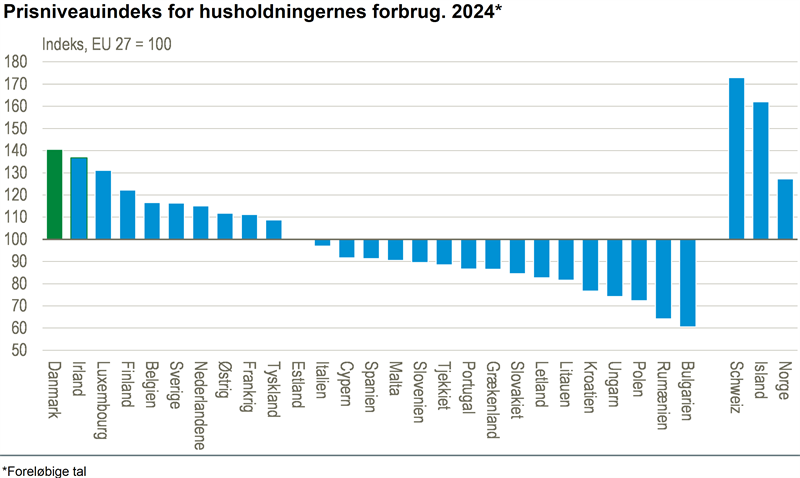
\includegraphics[width=0.8\textwidth]{assets/prisindeks.png}}
    \caption{Leveomkostninger i Danmark \footfullcite{Leveomkostninger2024}}
\end{figure}


\subsection{Abonnementers psykologiske effekter \label{sec:abpsef}}
Ud fra artiklen ”Understanding Subscription Models: \textit{»How Psychology Shapes
Customer Loyalty, Value Perception, and Cancellation Patterns«} \footfullcite{UnderstandingSubscriptionModels2025}, danner forfatteren et indblik i, hvordan strørre virksomhedder anvender psykologi til at påvirke, hvordan du opfatter dit abonnement, til at give dig en falsk fornemmelse af værdi. I artiklen bliver der beskrevet, hvordan personligt indforståelse af værdi påvirker individers sandsynlighed for at opsige et abonnement.

F.eks. grupperer virksomheder flere forskellige servicer som f.eks. streaming og musik + levering for en bestemt månedlig pris. Dette eksempel giver dig en fornemmelse af værdi for en højere pris. Dog bliver disse strategier primært anvendt for at give dig en fornemmelse af værdi, selv hvis du ikke anvender de yderligere grupperede fordele. I følgende analyse på næste side, kan det f.eks. ses, hvordan personer med abonnenter opfanger værdig, samt hvad der påvirker sandsynligheden for at opsige et abonnement ud fra den service som abonnementet tilbyder.

Ud fra Tabel 1 kan det ses, at de grupperede ydelser får procenten af folk til at opsige deres abonnementet ned på 12\% opsigelses lyst. Her ses det ligeledes, at forekommende prisstigninger har en opsigelses intention på 37\%, hvilket desuden er en af rødderne til vores nøgleproblem: Subscription fatigue.

\begin{table}[H]
\centering
\begin{tabularx}{\textwidth}{
    >{\raggedright\arraybackslash}X   % first column: left aligned flexible
    >{\centering\arraybackslash}m{3cm} % second column: centered fixed width
    >{\centering\arraybackslash}m{3cm} % third column: centered fixed width
    >{\raggedright\arraybackslash}X   % last column: flexible again
    }
    \toprule
    \rowcolor{gray!15}
    \textbf{Subscription Design} & 
    \textbf{Average Value Rating (1–5)} & 
    \textbf{Cancellation Intent (\%)} & 
    \textbf{Observed Psychological Effect} \\
    \midrule
    Bundled Services & 4.3 & 12\% & Framing $\rightarrow$ Enhanced Value \\
    Standalone Premium Tier & 3.7 & 24\% & Fairness Evaluation \\
    Frequent Price Increases & 3.1 & 37\% & Negative Affect, Loss Salience \\
    \bottomrule
\end{tabularx}
    \caption{Perceived Value by Subscription Design \footfullcite{UnderstandingSubscriptionModels2025}}
\end{table}

Både ud fra nogle forskellige strategier til at få folk til at beholde deres abonnementer.

Du kan se de Grupperede Ydelser får procenten af folk til at opsige deres abonnoment
ned på 12\% opsigelses lyst, hvor at forkommende pristigninger har en opsigelses
intetion på 37\%, dette er en af røderne til vores nøgle problem: Subscription fatigue

Herefter har vi også en virksomheds baseret grådighed, ved abonnomenter ejer du
aldrig det du betaler for, hvilket vil sige at virksomhederne har 100\% ejerskab over det
produkt du har købt.

I artiklen “The Subscription Economy and Its Contribution to the Global Economy” skrevet af Paula Cobazaru, som er Assistant Professor, phd studerende ved Alexandru Loan Cuza University Og Alexandru Tugui, som er professor ved Alexandru Loan Cuza University
bliver der beskrevet, at gennemsnitligt betaler den individuelle forbruger 133\$ om måneden på abonnementer som vil svare til 853,43 DKK om måneden, hvilket svarer til ca 10266,79 DKK om året pr. forbruger, med en estimeret stigning på 18\% om året. Og hvis man så tager det til sammenligning til hele jordens befolkning, vil det lægge den estimerede markedsværdi inden for abonnementer på cirka 1,5 trillion dollars, eller 9.624.300.000.000 DKK.

Hvilket betyder abonnementer har fået en meget større økonomisk og global betydning, og at den globale markedsværdi konstant vil stige.

Da virksomhederne får muligheder for at styre udbud og efterspørgelse selv, kan de selv styre hvor meget der ryger ind og ud af markedet. Dette danner et kæmpe problem for den gennemsnitlige forbruger, da individet ikke har noget ejerskab eller kontrol. Virksomheder kan også bruge disse abonnementer til at danne faste relationer med kunderne, hvilket gør at individet har svære ved at få kontrol over egen kapital. Dette fører derfor til Subscription fatigue, hvor individet ikke har nogle form for overblik over deres abonnementer og økonomi til et punkt hvor forbrugeren ikke agerer på deres økonomi længere.


\subsection{Subscription fatigue}
Subscription fatigue på dansk »abonnementsudmattelse«, som er den mentale og økonomiske tilstand, der opstår, når en forbruger føler sig overvældet af antallet af løbende betalinger og tjenester, som de skal administrere. I denne rapport anvender vi begrebet som en »diagnose« af et moderne samfundsproblem, hvor den teknologiske udvikling har gjort det for nemt at starte et abonnement, men for uoverskueligt at vedligeholde eller opsige det.


Hvorfor opstår Subscription fatigue? 


Subscription Fatigue opstår typisk på grund af tre hovedfaktorer:\footfullcite{subFatt}
\begin{enumerate}
    \item \textbf{Kognitiv overbelastning:}\\
    Forbrugeren mister overblikket over, hvilket tjenester de reelt har adgang til, og hvilket de bruger. Når hver tjeneste kræver sit egent login, app og betalingsaftale, ophører abonnementet med at være en bekvemmelighed og bliver i sted et en administrativ byrde. 
    \item \textbf{Økonomisk »leaking«:}\\
    forbrugeren oplever små månedlige beløb, som virker ret ubetydelige hver for sig, men samlet så dræner de privatøkonomien (jf. afsnit \ref{sec:abpsef} om det gennemsnitlige forbrug på 853 kr./md.). Dette skaber helt underbevidst en stressfaktor, da man ved, pengene forsvinder til forbrug, men ikke præcis hvorhen.
    \item \textbf{Beslutningslammelse:}\\
    Som beskrevet i afsnit \ref{sec:abpsef}, bruger virksomheder psykologiske tricks som bundling. Dette gør det svært for brugeren at vurdere den reelle værdi af tjenesten, hvilket fører til, at man beholder et abonnement "for en sikkerheds skyld", selvom man sjældent bruger det. 
\end{enumerate}
 
Vores fokus i dette projekt er ikke blot at identificere Subscription fatigue, men at udvikle et teknologisk værktøj, der kan hjælpe med at modkæmpe det. Ved at automatisere overblikket kan vi fjerne den kognitive belastning fra individet og derved forbedre både deres økonomiske råderum og deres livskvalitet.
     
    
    
    % Bibliografi
    \newpage
    \nocite{*}
    \printbibliography[heading=bibintoc,title={Litteraturliste}]

    % Appendiks
    \newpage
    \begin{appendices}
        \section{Appendiks}
        \section{HV-modellen}
\label{apx:hv-modellen}
Vi anvender her HV-Modellen til at gå i dybden med Subscription-Fatigue 

\textbf{Hvad?} 

\begin{itemize}
\item Hvad skal man gøre? 
\item Subscription-Fatigue, primært hvis du bliver udsat for subscription-fatigue, er de hyppigste løsninger at lave en list og danne overvejelser over hvilket du bruger og hvilket du ikke bruger. 
\item Hvad bliver gjort? 
\item Mange bliver bare ved med at betale for deres abonnementer, og kigger ikke efter billigere løsninger, som medfører til et økonomisk tab 
\item Hvad burde blive gjort? 
\item Der burde blive undersøgt efter troværdighed på firmaet du har et abonnement på, herefter undersøg hvor vidt det indeholder hvad du skal bruge, og hvad du ikke bruger. 
\item Undersøg hvordan du også kan finde billigere alternativer til hvad du har abonnementer indenfor. Da grupperede abonnementer hyppigst er billigere. 
\item Hvad kan ellers gøres? 
\item Opsige abonnementet, hvis det ikke har nogle nyttighed 
\item Hvad burde ellers blive gjort? 
\item Opsætte en fast dag, eks hvert 3 måned hvor du gennemgår dine abonnementer igen, og undersøger sine abonnementer igen. 
\end{itemize}

\textbf{Hvorfor?}
\begin{itemize}
    \item Hvorfor gør han/hun det? 
    \item Subskription fatigue forekommer hyppigst, når vedkommet, ikke holder styr på deres abonnementer og ikke framælder dem når de ikke bruger dem. 
    \item Det bygger så op i økonommien og til sidst kan vedkommet ikke huske hvor de mælder dem fra 
    \item Hvorfor gøre det?     
    \item Personen vælger oftest et abonnement, frem for 1gangs betaling, fordi de virker billigre over den korte periode, men senere hen bliver dyt, ellers ligger det på et punkt hvor individet ikke har 1 gangsbeløbet men har råd til at tage et subsciption hvor du afbetaler over længere perioder. 
\end{itemize}
    
\textbf{Hvem?}
\begin{itemize}
    \item Hvem gør det? 
    \item Det er typisk, ældre puplikum som falder i abonnomenter, som Telefon abonnoment, tv abonnoment, Lån, elregninger, telefon apps. 
    \item Som trækker på din økonomi månedligt. 
\end{itemize}

\textbf{Hvornår?}
\begin{itemize}
    \item Hvornår skal man gøre noget ved det? 
    \item Subscription fatigue skal behandles så snart du kan mærke økonomiske fald, så dine økonomiske tab kan minimeres hurtigst muligt 
    \item Hvornår kan det ellers blive gjort? 
    \item Du kan gøre noget ved det, men hvis du kan få gjort noget ved det hurtigst muligt vil det minimere skaderne. 
\end{itemize}

\begin{landscape}
    \section{Første skitse af applikation}
    \label{apx:dig_skitse_af_app}
    \begin{center}
        \fbox{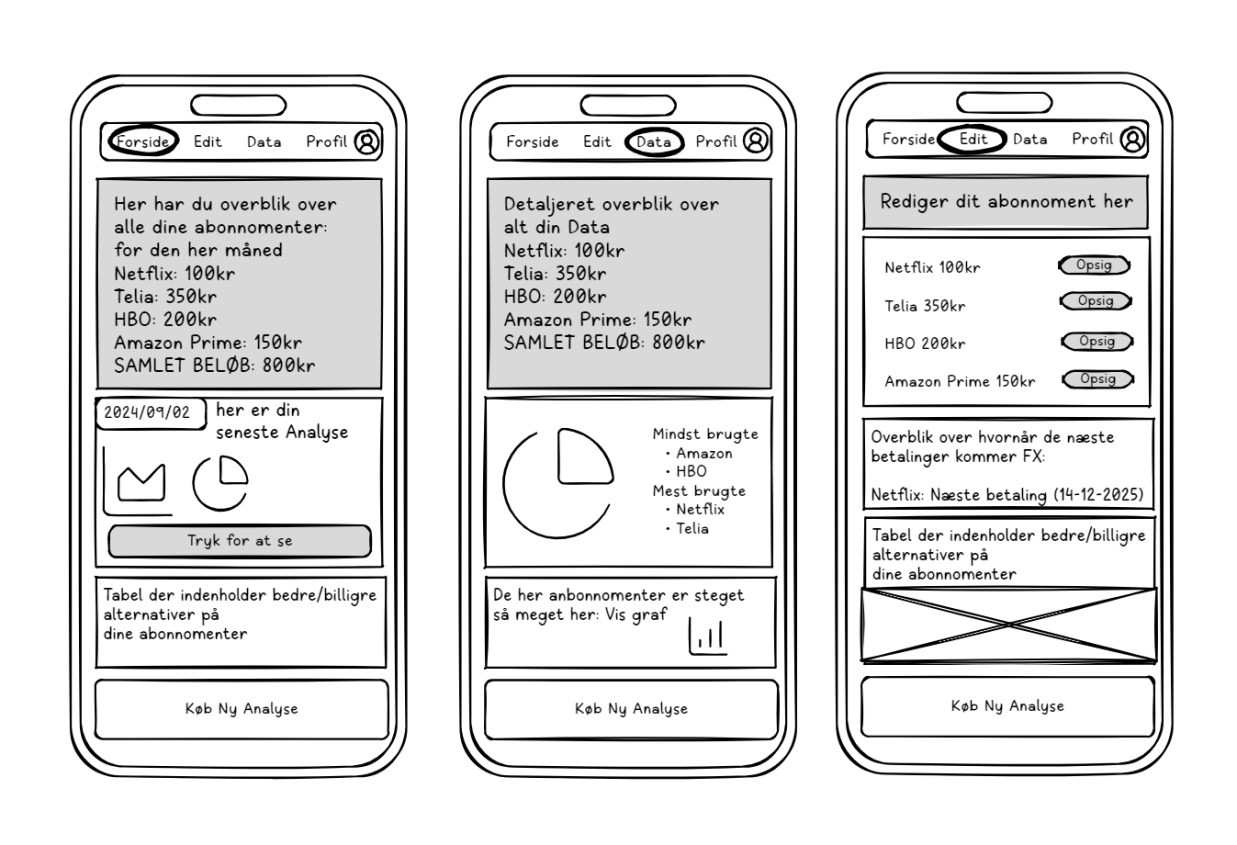
\includegraphics[width=0.8\linewidth]{../latex-document/assets/skitse_af_app.png}}
    \end{center}
\end{landscape}

\newpage

\section{skitse af navbar til a/b test}
\textbf{A version af navigationsbjælken}
  \begin{figure}[H]
    \label{apx:navbar_ab_test}
    \centering
    \fbox{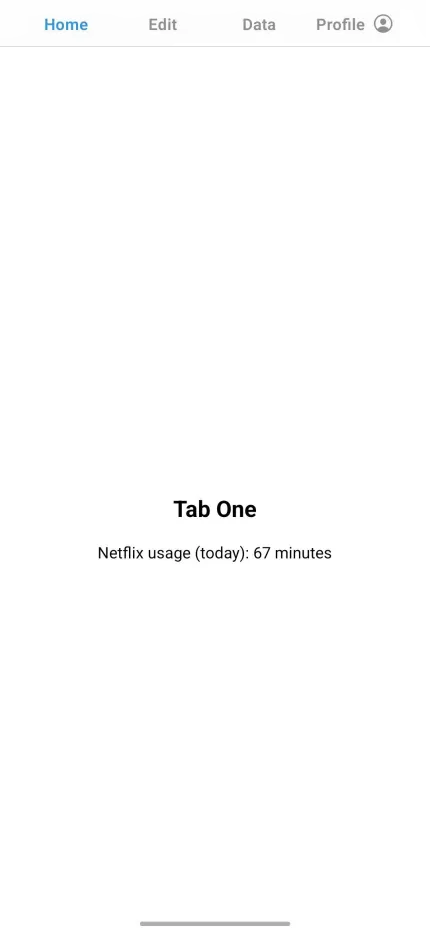
\includegraphics[width=0.5\textwidth]{assets/proto_0001_home.png}}
    \caption{A version af navigationsbjælken}
  \end{figure}

  \textbf{B version af navigationsbjælken}
  \begin{figure}[H]
    \centering
    \fbox{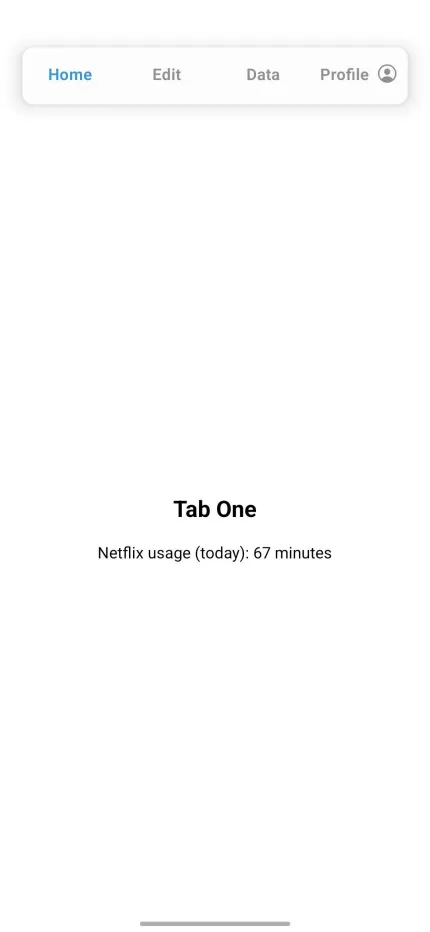
\includegraphics[width=0.5\textwidth]{assets/proto_1_home.png}}
    \caption{B version af navigationsbjælken}
  \end{figure}

\newpage
\section{Skærmbillede af data-side}
\begin{figure}
    \centering
    \fbox{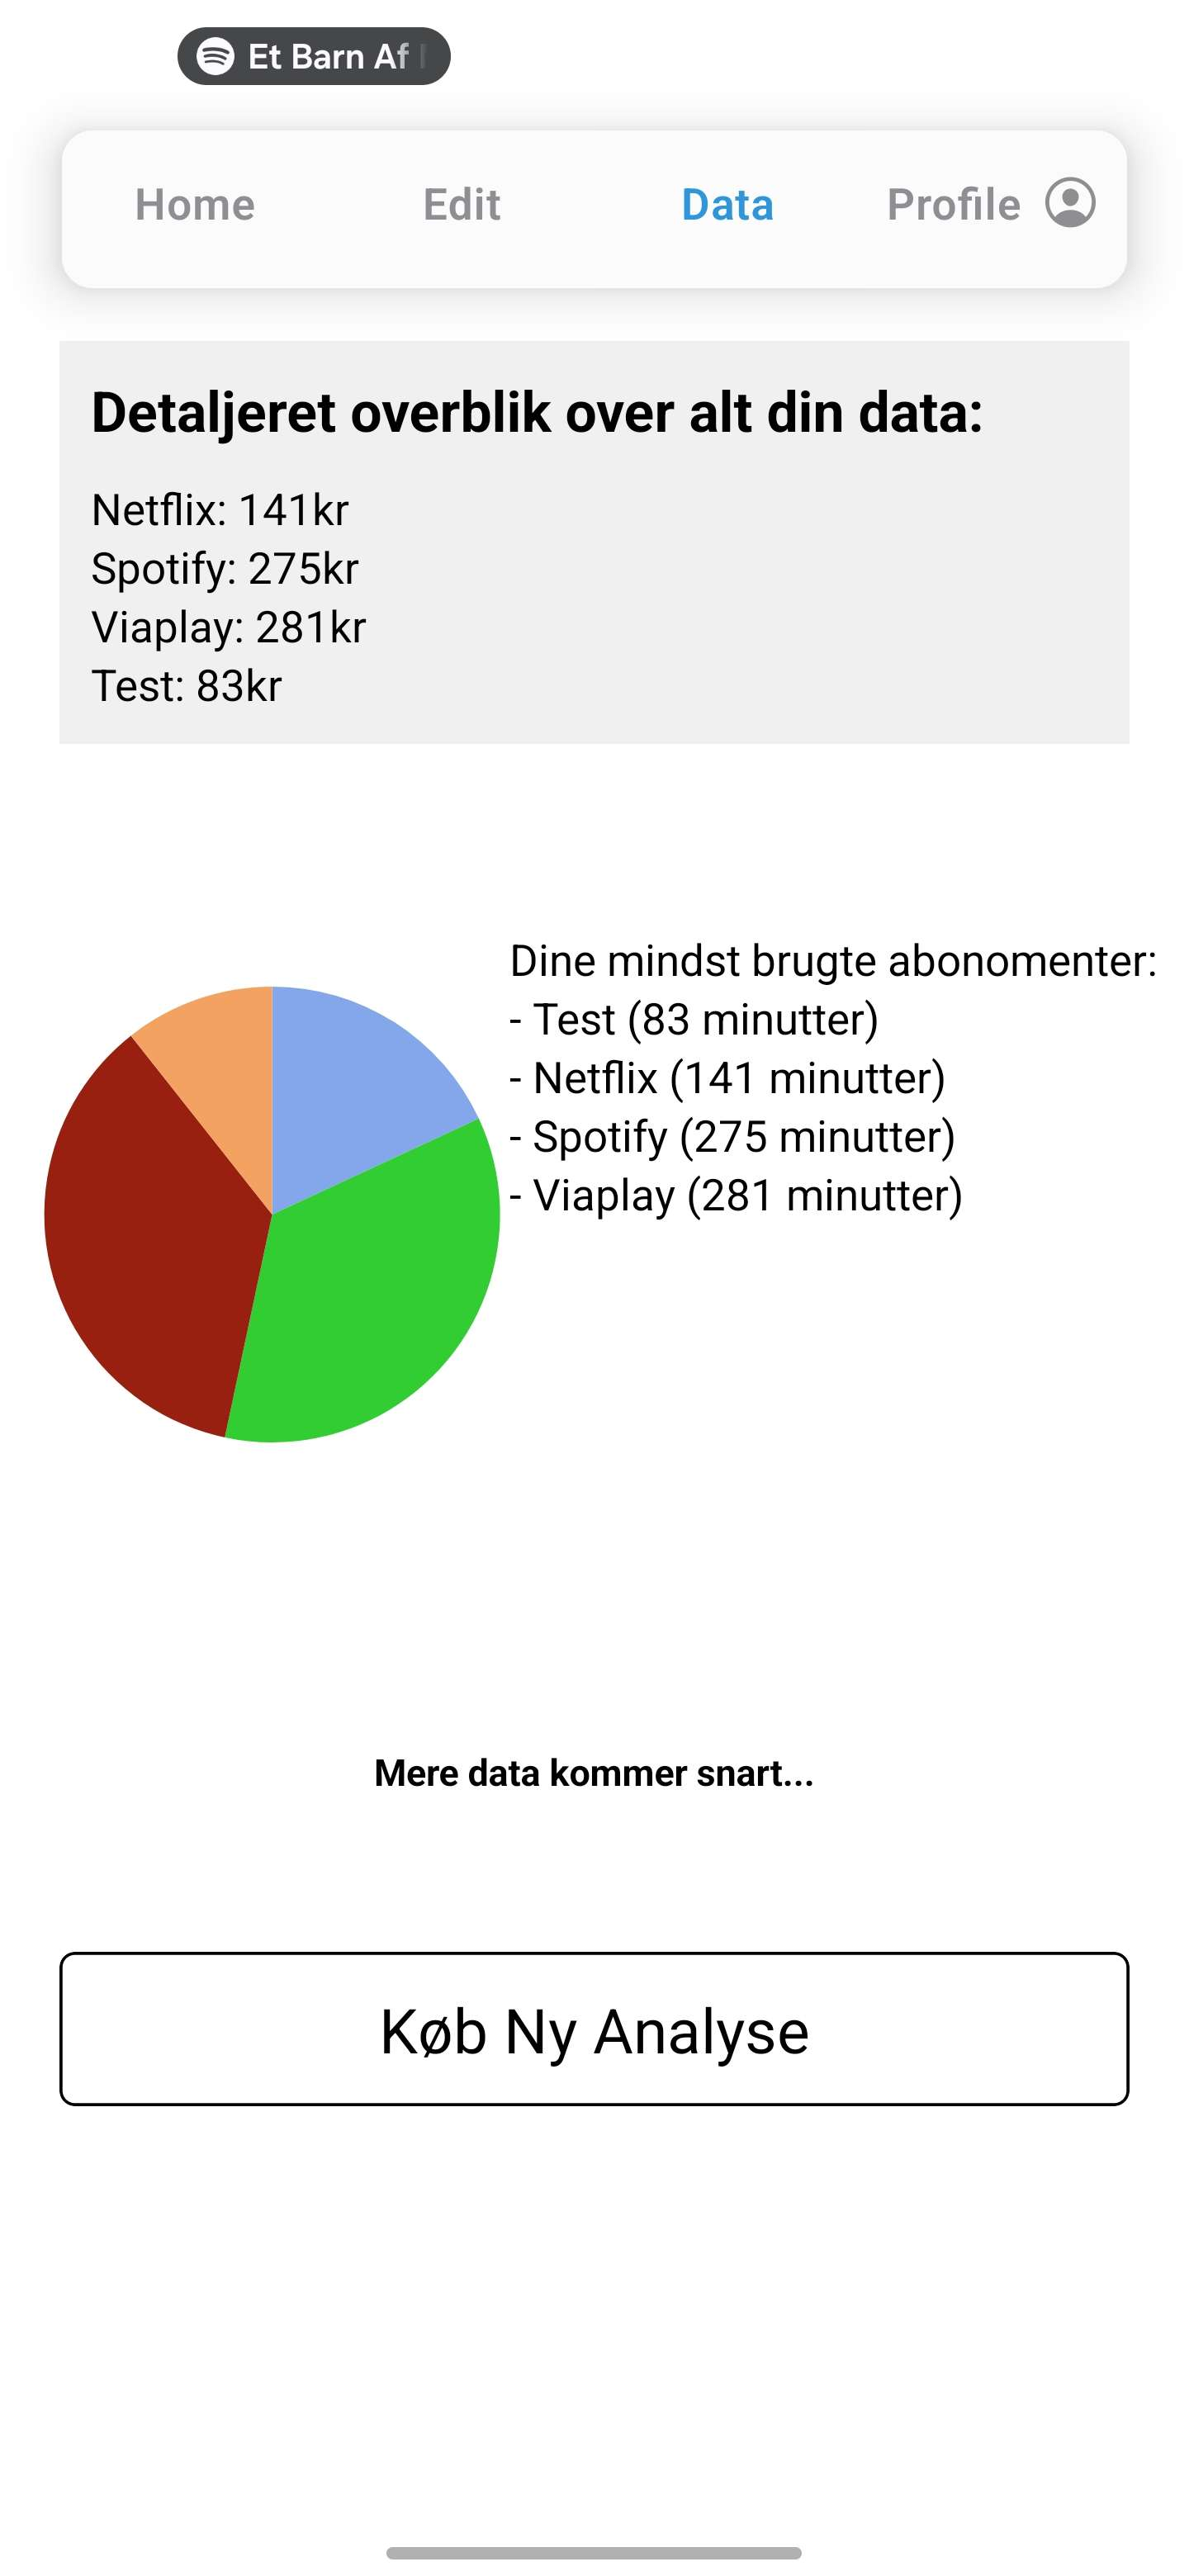
\includegraphics[width=0.5\textwidth]{assets/data_page_graph.jpg}}
    \caption{Skærmbillede af data-side}
\end{figure}

\newpage
\section{Kildekode dataindsamling}
\label{apx:getUsage}
\begin{mdframed}[backgroundcolor=blue!5]
\begin{minted}[breaklines]{tsx}
import * as UsageStats from 'expo-android-usagestats';
import { Alert, Linking, Platform } from 'react-native';


export async function ensureUsagePermission(): Promise<boolean> {
  if (Platform.OS !== 'android') return true;

  try {
    const has = await UsageStats.hasUsageStatsPermission();
    if (has) return true;

    await UsageStats.requestUsageStatsPermission();

    const hasAfter = await UsageStats.hasUsageStatsPermission();
    if (hasAfter) return true;

    Alert.alert(
      'Usage access required',
      'This feature needs Android Usage Access to read app foreground times. Open settings to grant access?',
      [
        { text: 'Cancel', style: 'cancel' },
        {
          text: 'Open Settings',
          onPress: () => {
            Linking.openSettings().catch(() => {});
          },
        },
      ]
    );

    return false;
  } catch (err) {
    console.warn('Error checking/requesting usage permission', err);
    return false;
  }
}


export async function getUsageForPackage(packageName: string, days = 1): Promise<
  { totalTimeInForeground: number; minutes: number } | null
> {
  const end = Date.now();
  const start = end - days * 24 * 60 * 60 * 1000;
  const stats = await UsageStats.getUsageStats(start, end);
  const needle = packageName.toLowerCase();

  const matches = stats.filter((app) => {
    if (!app || !app.packageName) return false;
    const pn = String(app.packageName).toLowerCase();
    const an = String((app as any).appName ?? '').toLowerCase();
    return pn === needle || pn.includes(needle) || an.includes(needle);
  });

  if (!matches || matches.length === 0) {
    console.log(`getUsageForPackage: no usage-stats entries matched '${packageName}' for ${days} day(s). Top packages:`);
    stats.slice(0, 20).forEach((s: any, i: number) => {
      const pn = s.packageName ?? s.package ?? '(unknown)';
      const ms = (s as any).totalTimeInForeground ?? (s as any).totalTimeForeground ?? (s as any).totalForegroundTime ?? (s as any).totalTime ?? 0;
      console.log(i, pn, ms);
    });
    return null;
  }

  const getMs = (s: any) => {
    return (
      s.totalTimeInForeground ??
      s.totalTimeForeground ??
      s.totalForegroundTime ??
      s.totalTime ??
      s.totalTimeForegroundServiceUsed ??
      0
    );
  };

  const totalMs = matches.reduce((acc: number, s: any) => acc + (Number(getMs(s)) || 0), 0);

  if (totalMs === 0) {
    console.log(`getUsageForPackage: matched entries for '${packageName}' but totalMs==0 for ${days} day(s). Matches:`);
    matches.forEach((m: any, i: number) => console.log(i, m.packageName, getMs(m), m));
  }

  const minutes = Math.round(totalMs / 60000);
  return { totalTimeInForeground: totalMs, minutes };
}
\end{minted}
\end{mdframed}

\newpage
\section{Skærmbilleder af produktet}
\begin{landscape}
\begin{figure}
  \fbox{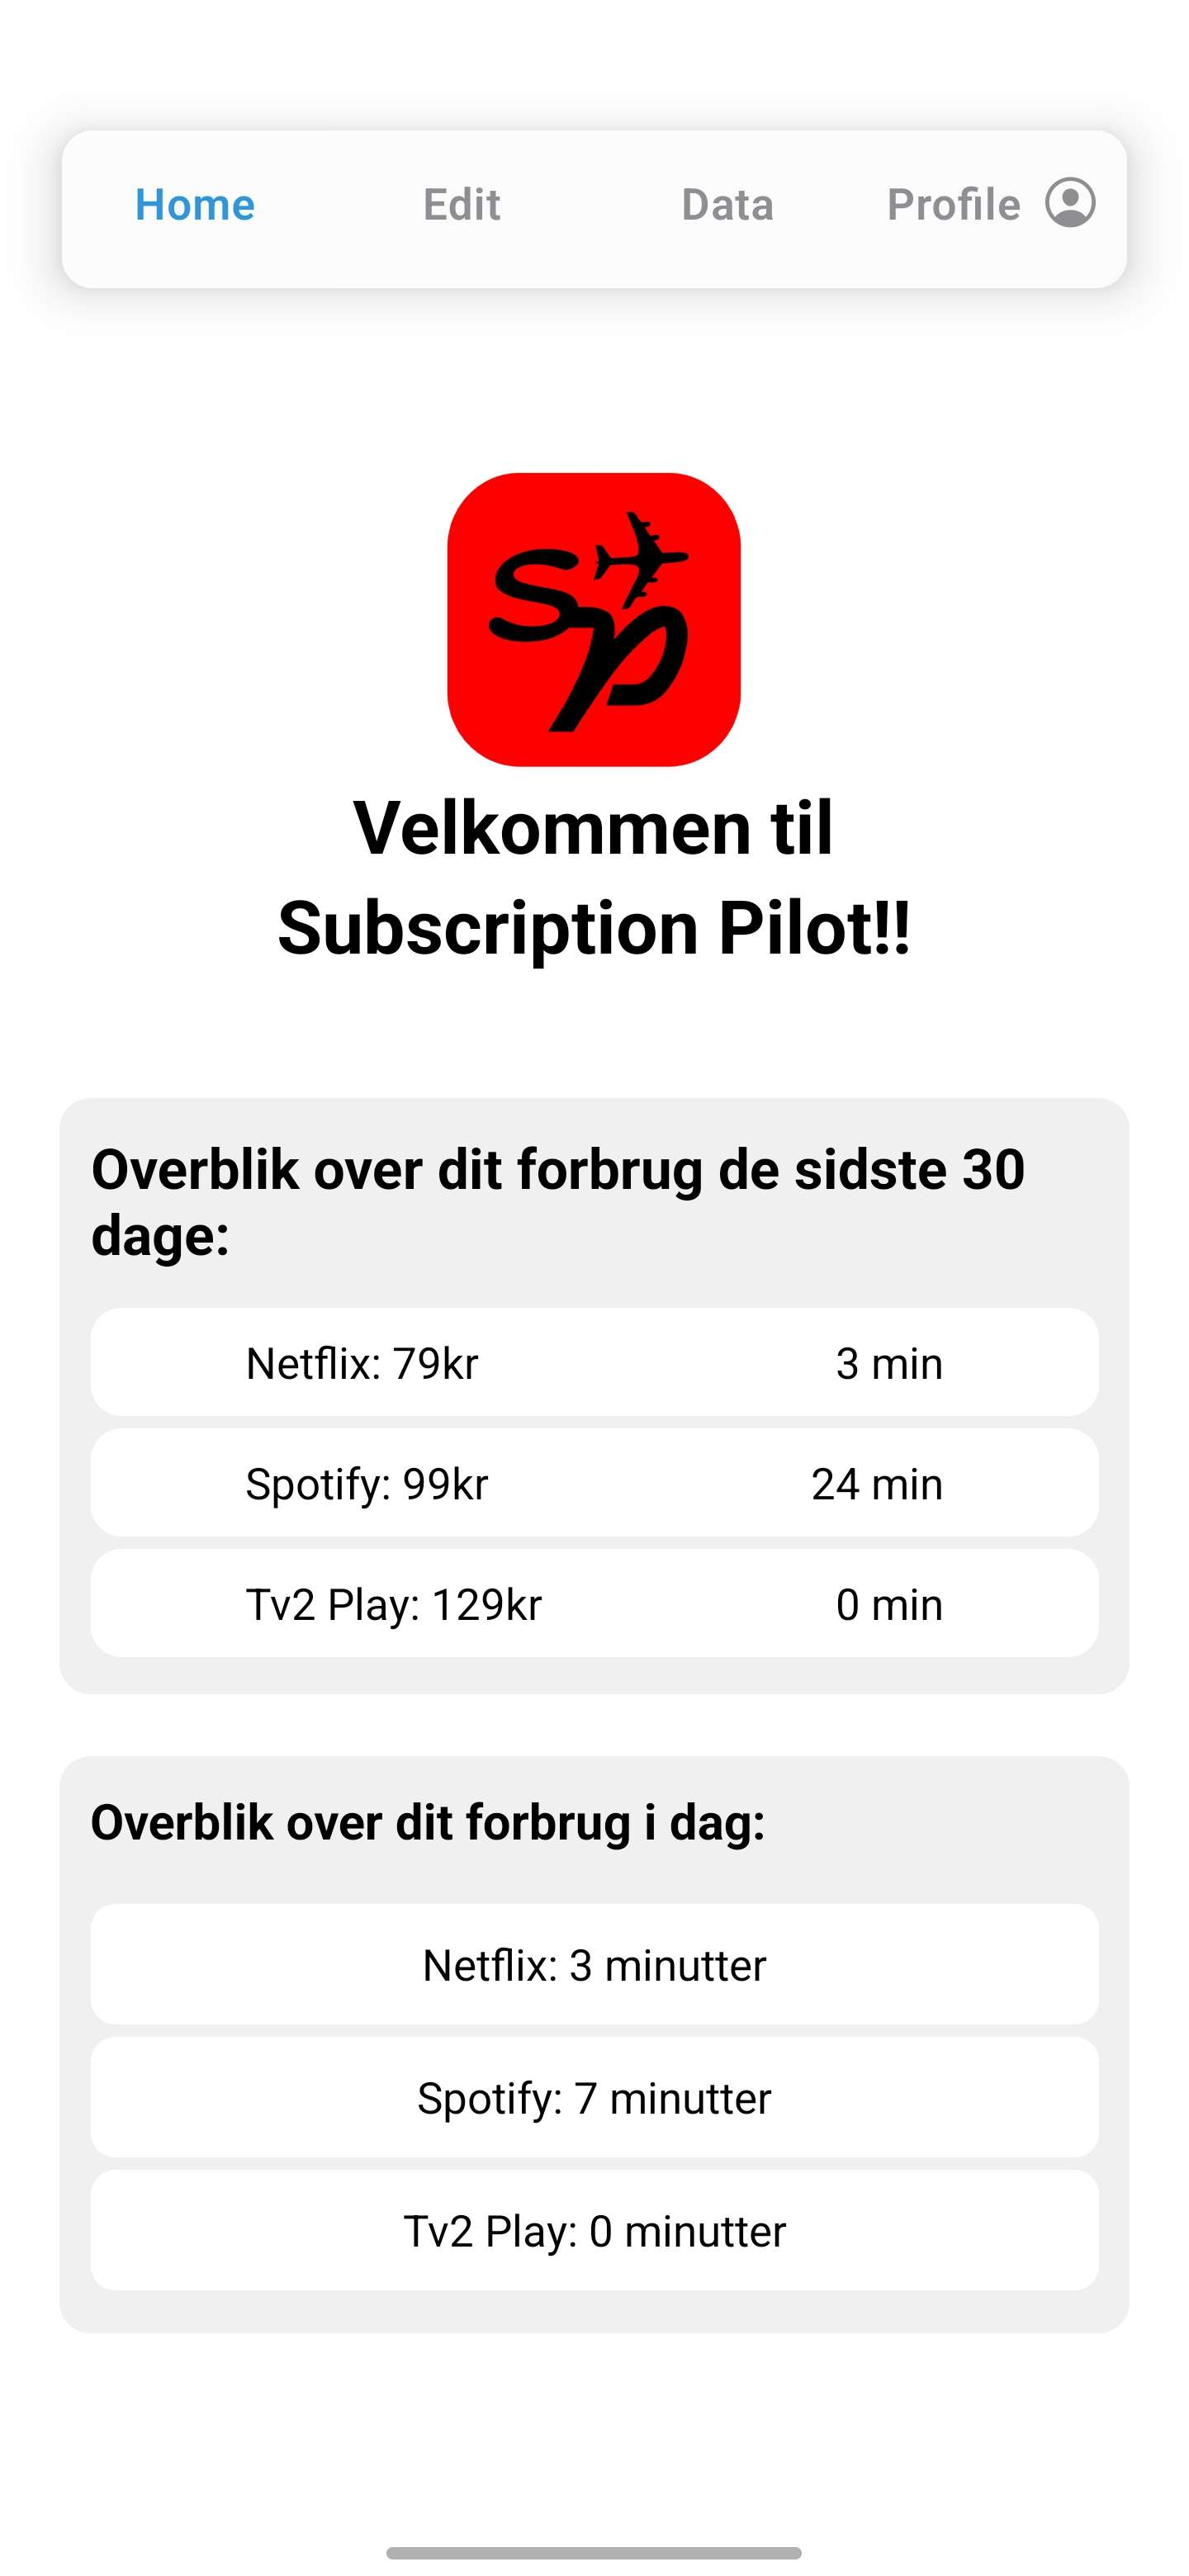
\includegraphics[width=0.5\textwidth]{assets/hifi-skitser/home-before-yt.jpg}}
  \fbox{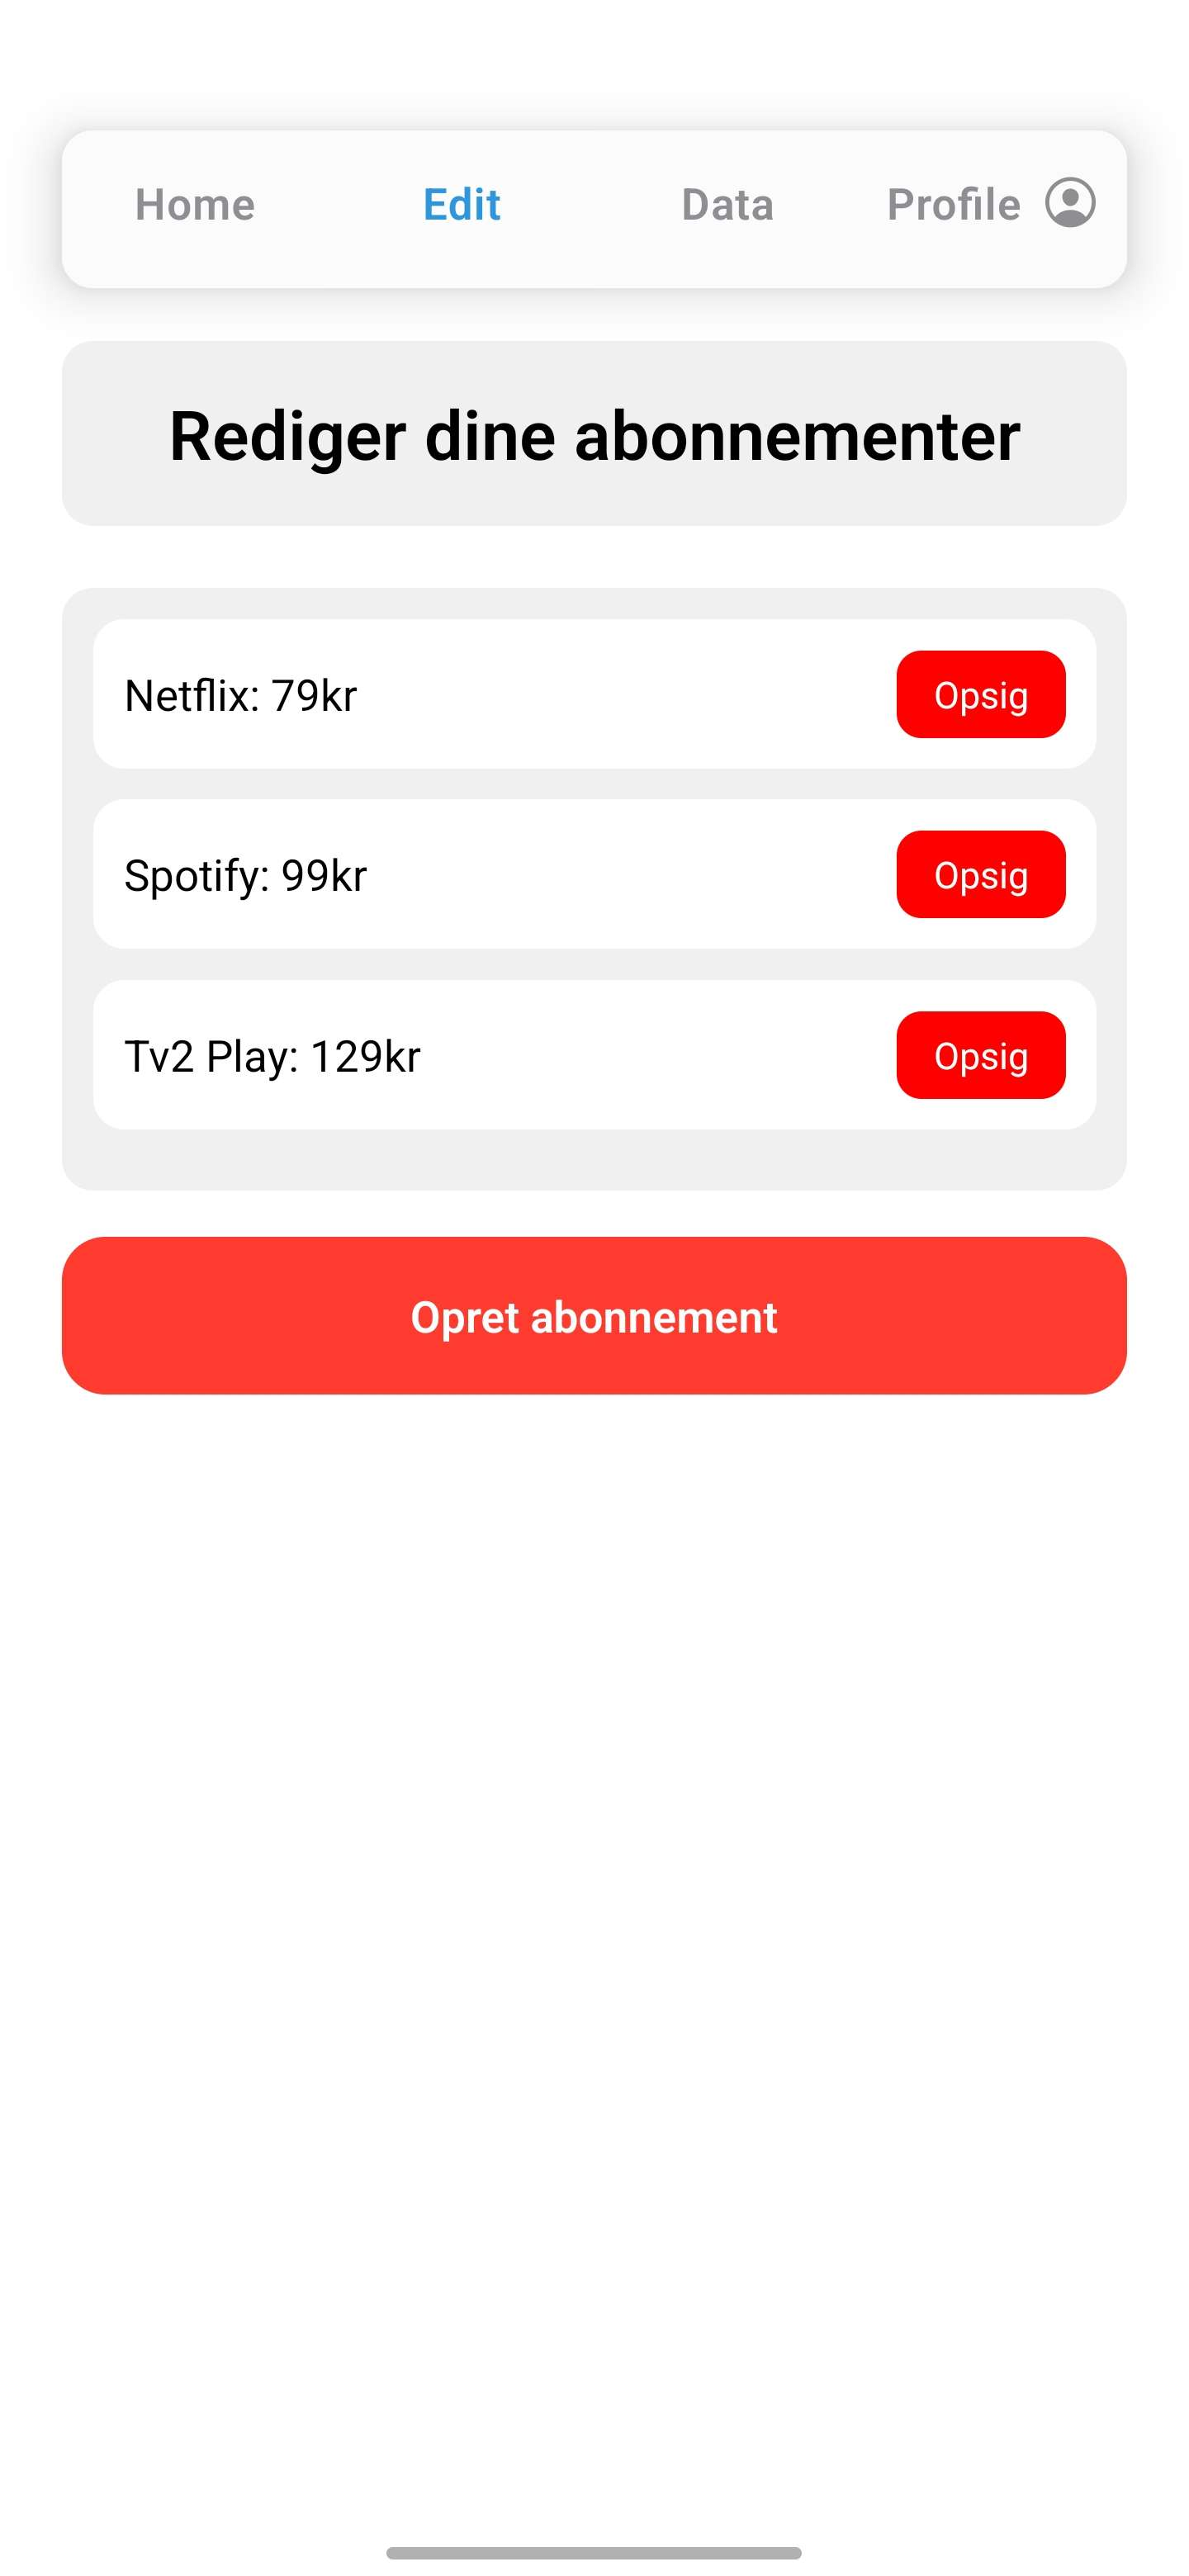
\includegraphics[width=0.5\textwidth]{assets/hifi-skitser/edit_before_yt.jpg}}
  \fbox{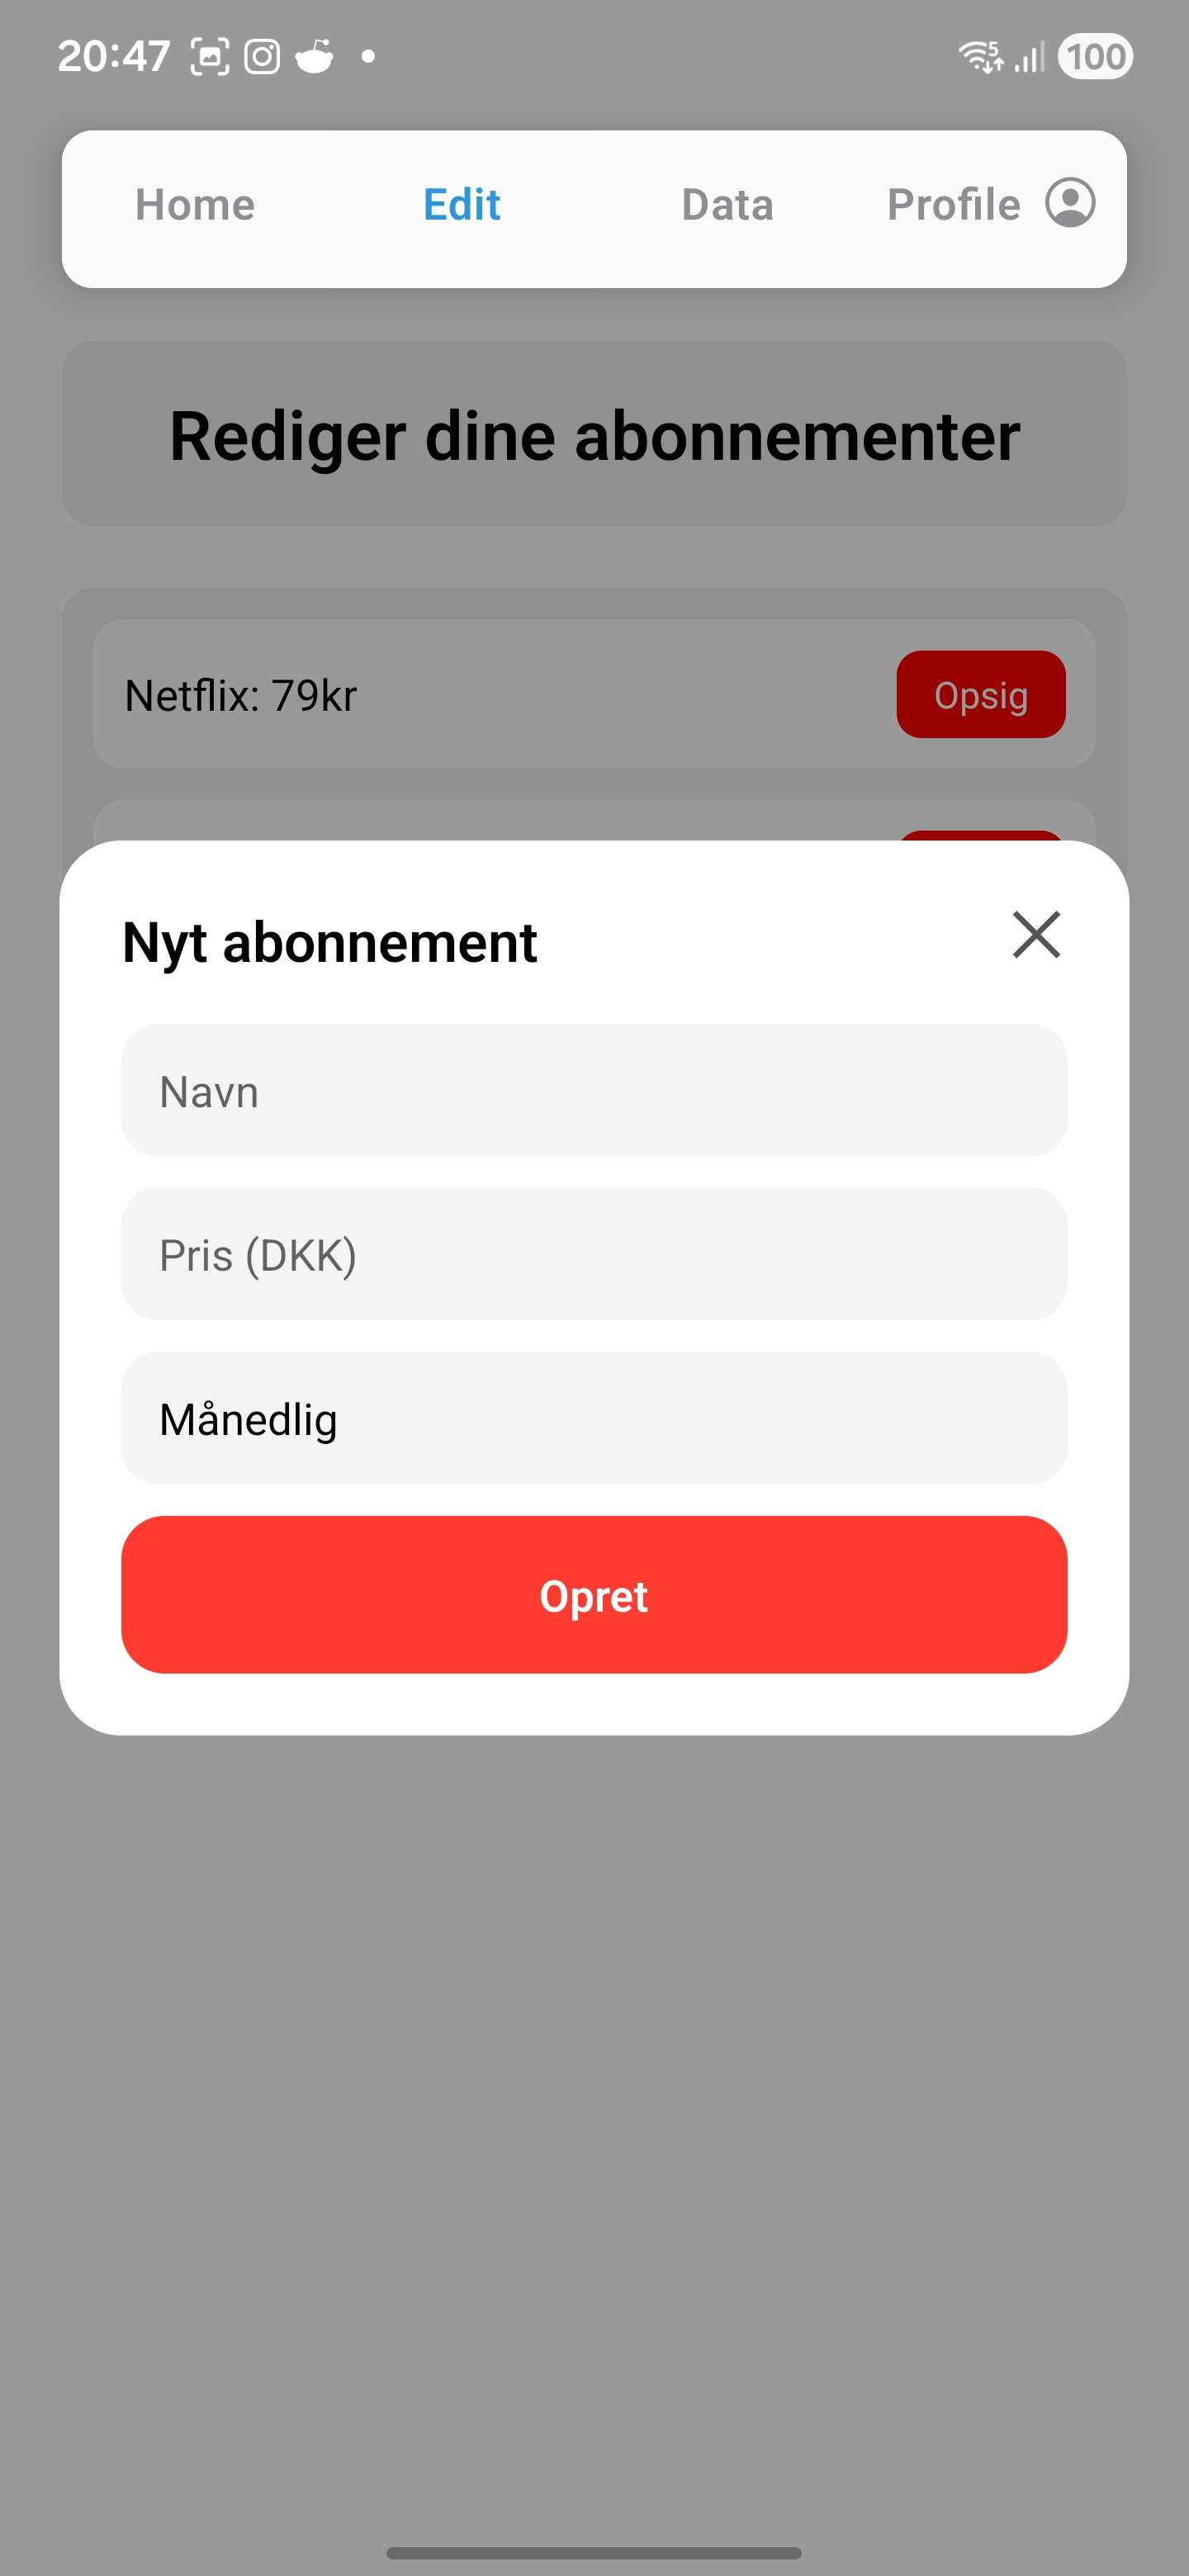
\includegraphics[width=0.5\textwidth]{assets/hifi-skitser/edit-opret.jpg}}
\end{figure}  
\end{landscape}

\begin{landscape}
  \begin{figure}
    \fbox{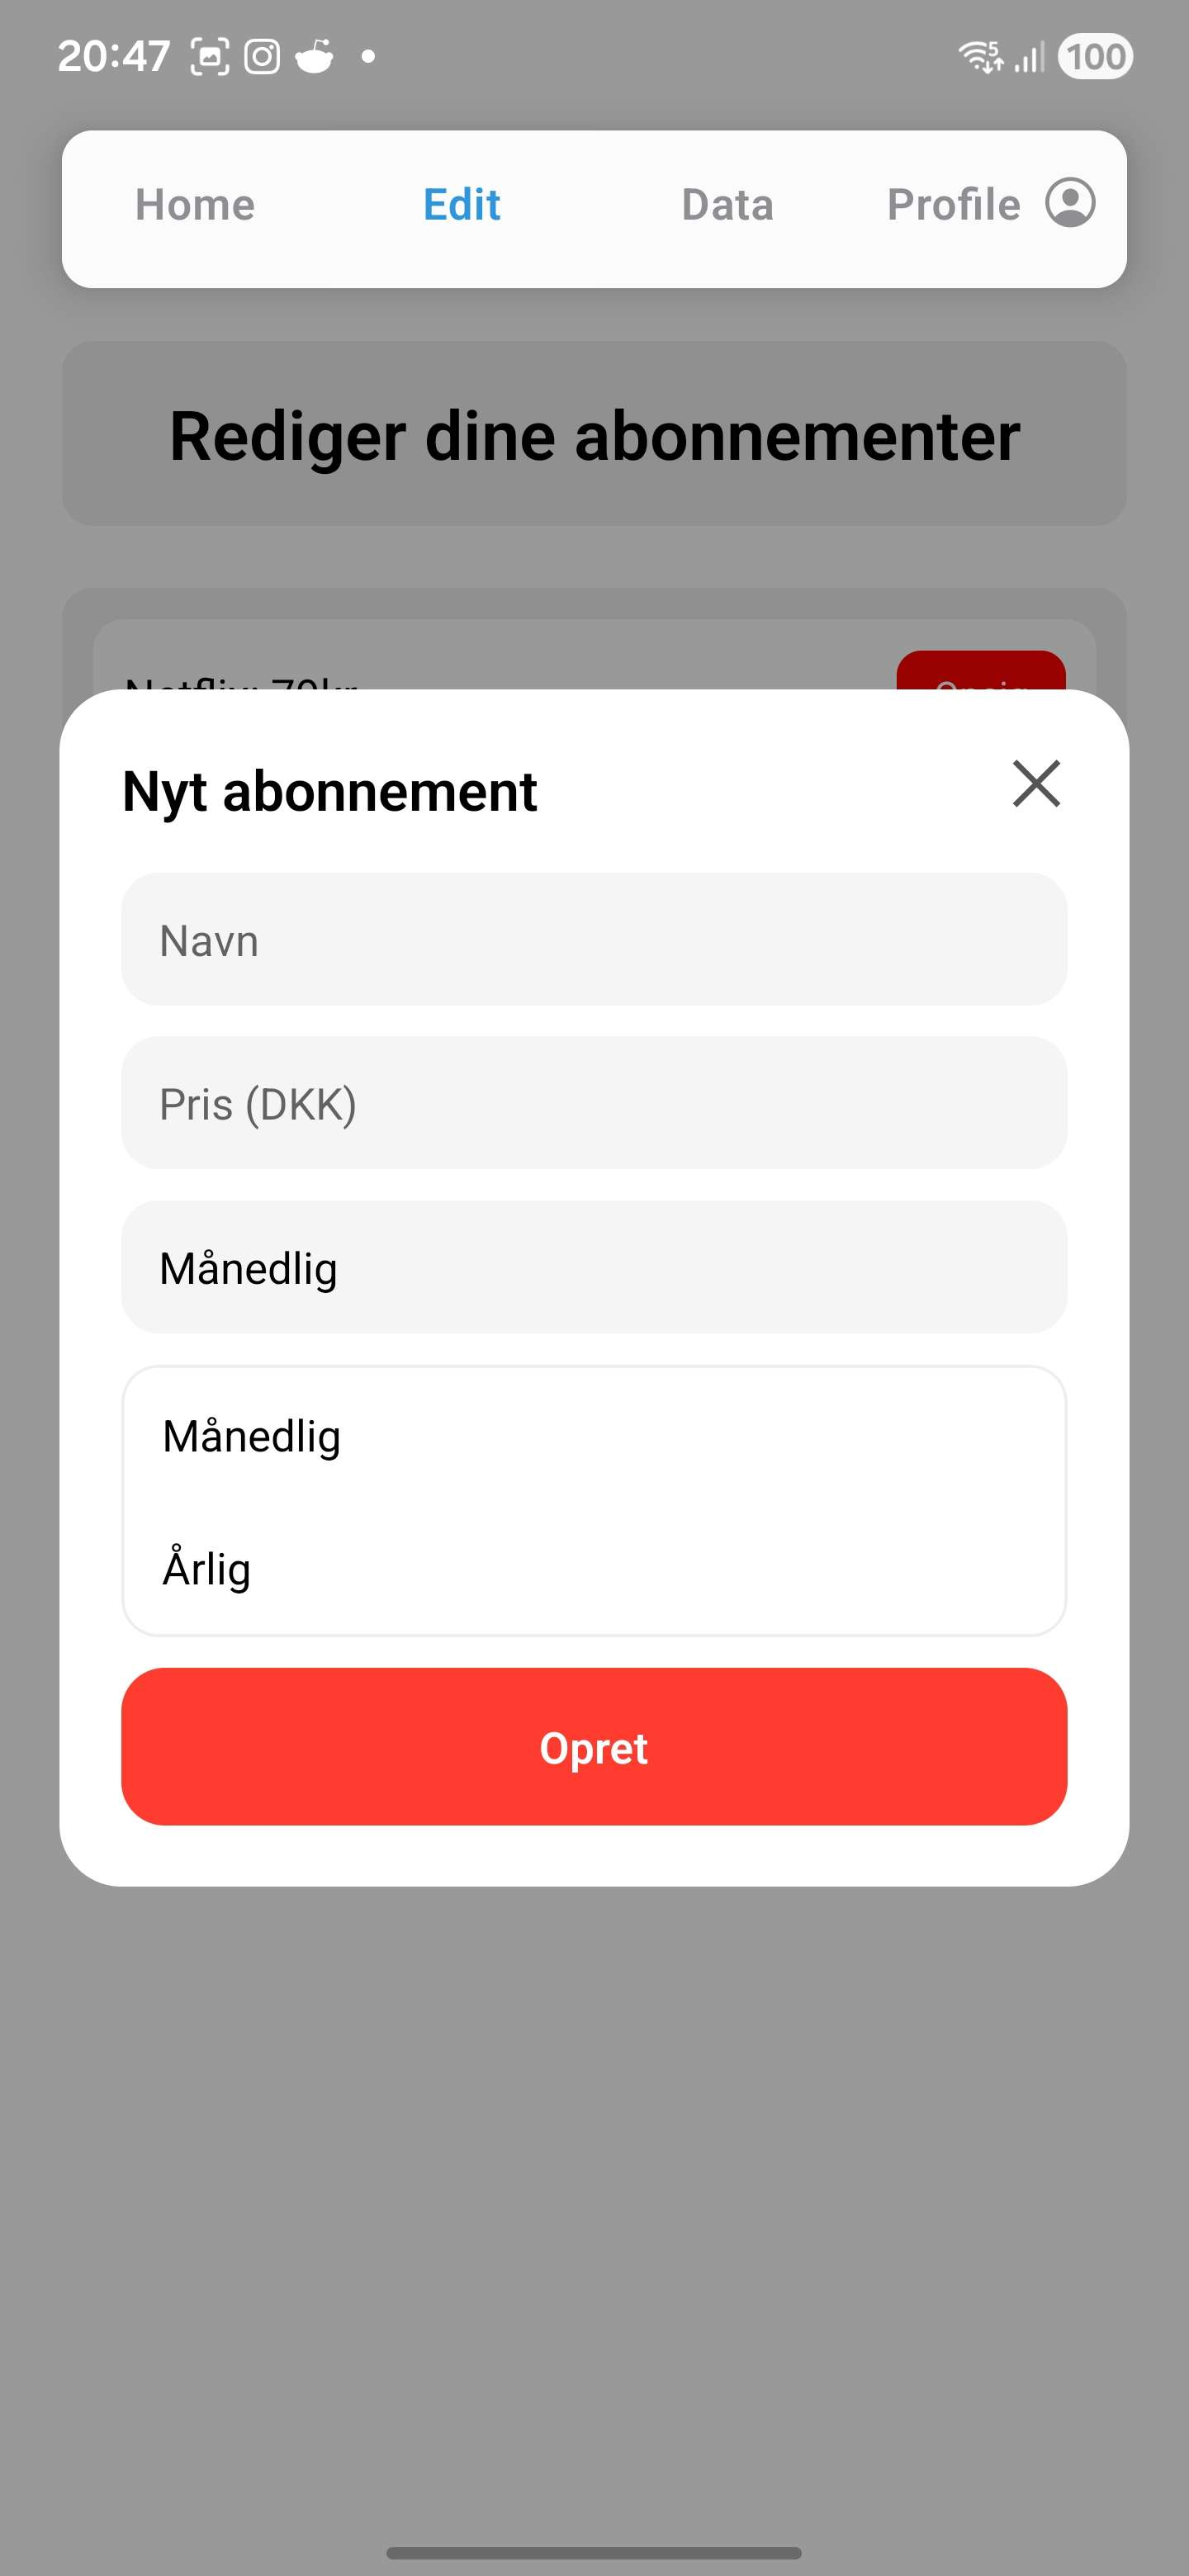
\includegraphics[width=0.5\textwidth]{assets/hifi-skitser/edit-opret-dropdown.jpg}}
    \fbox{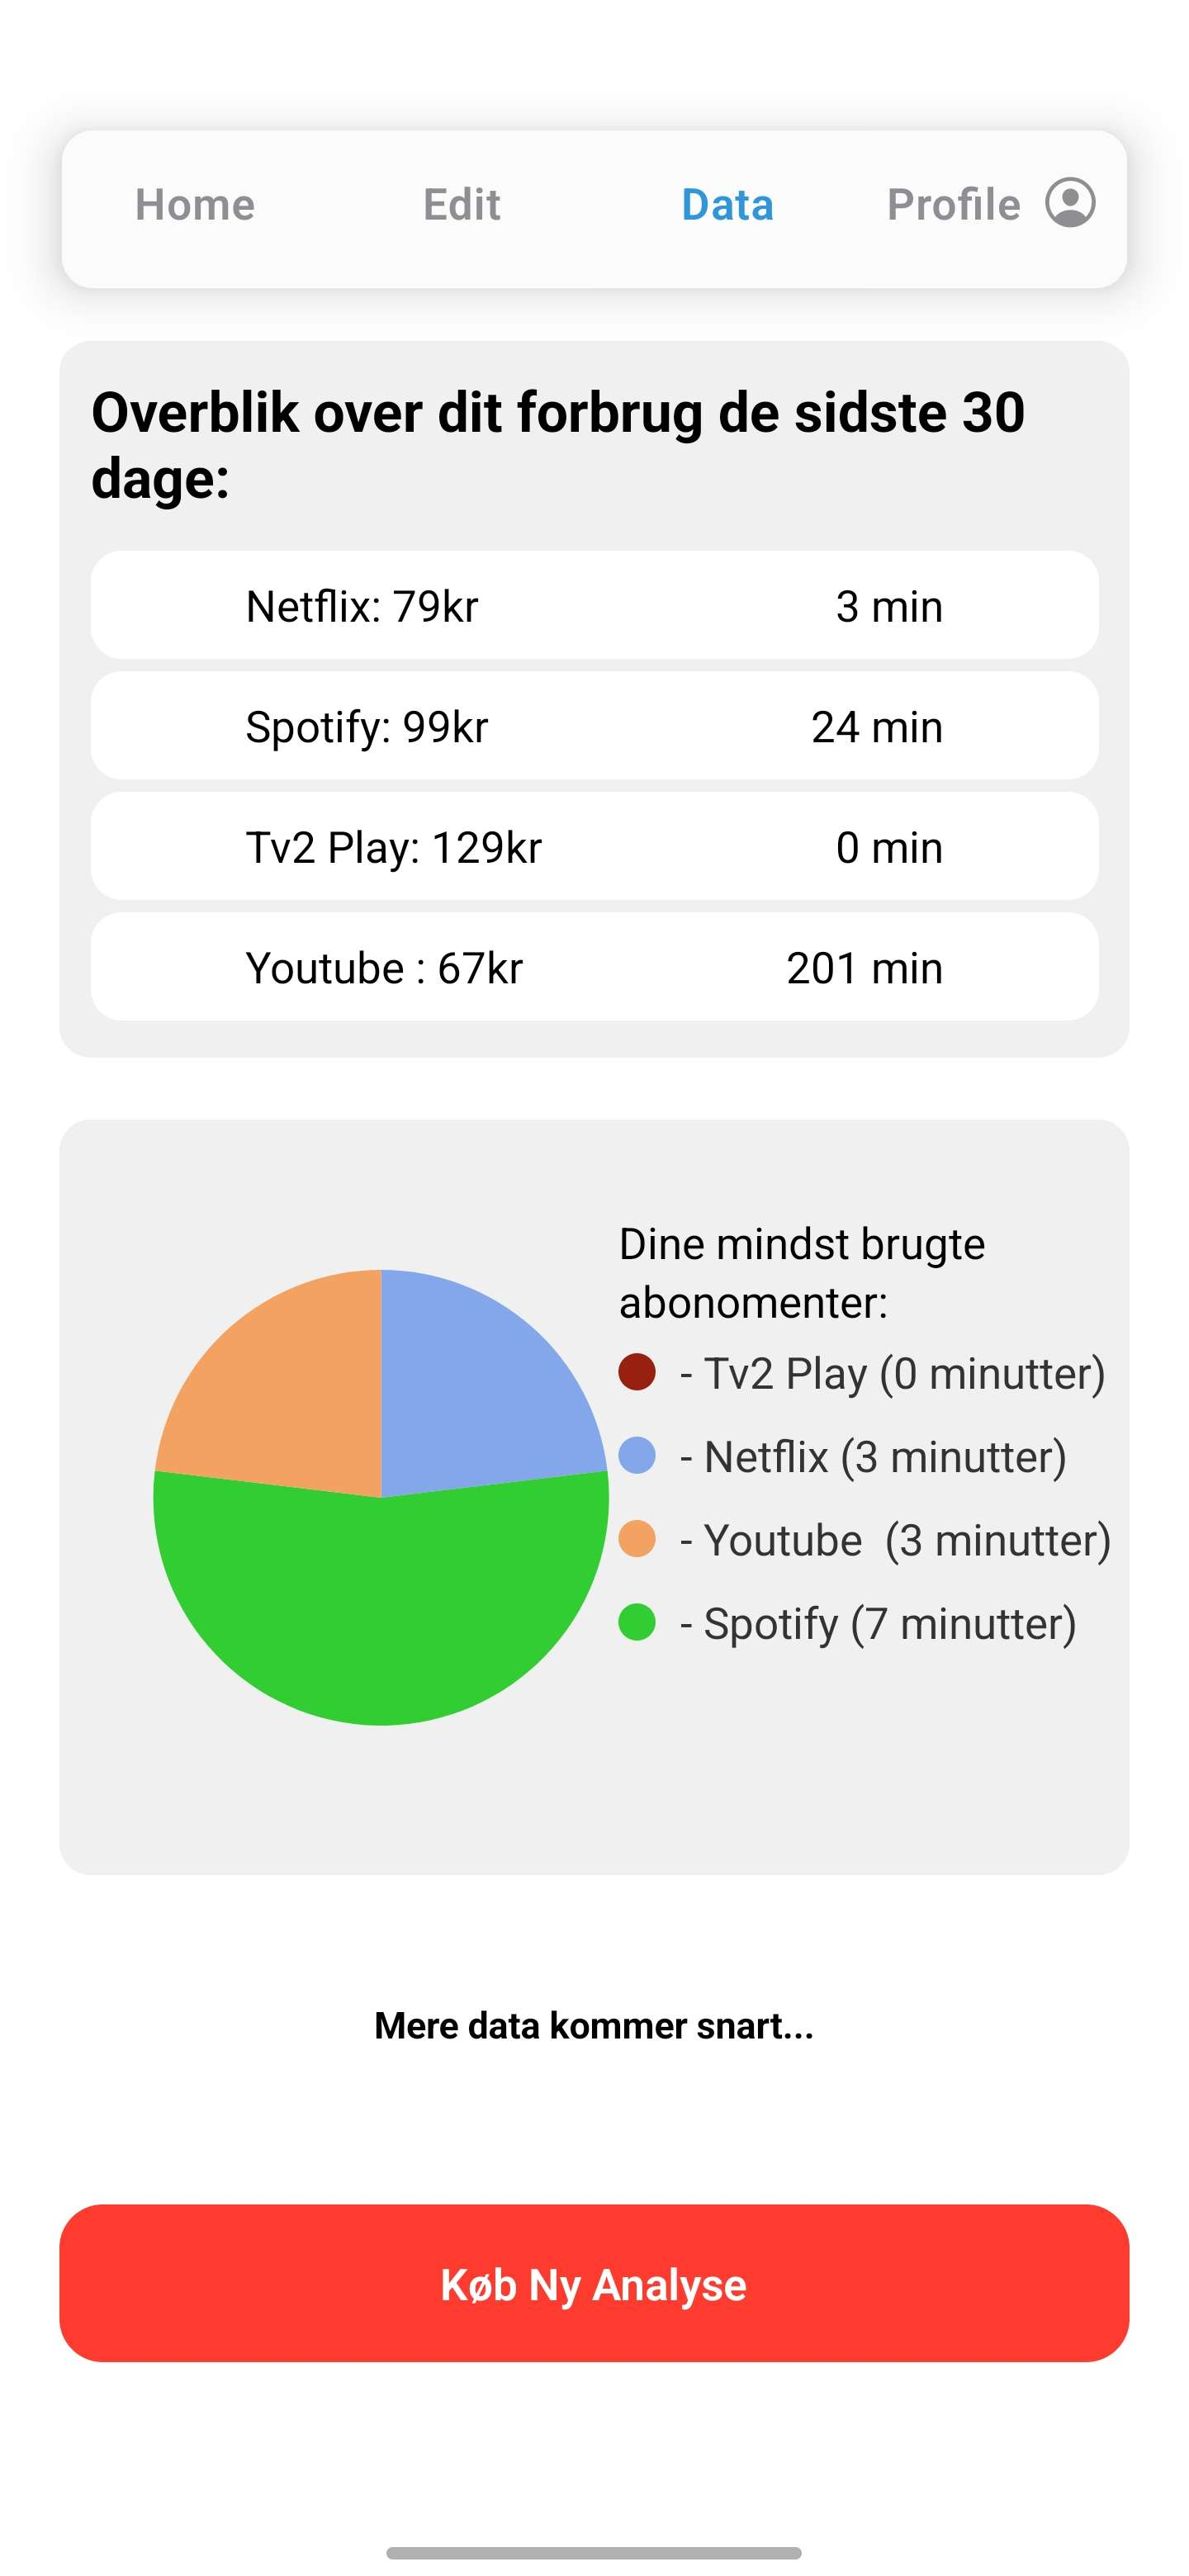
\includegraphics[width=0.5\textwidth]{assets/hifi-skitser/data-after-yt.jpg}}
    \fbox{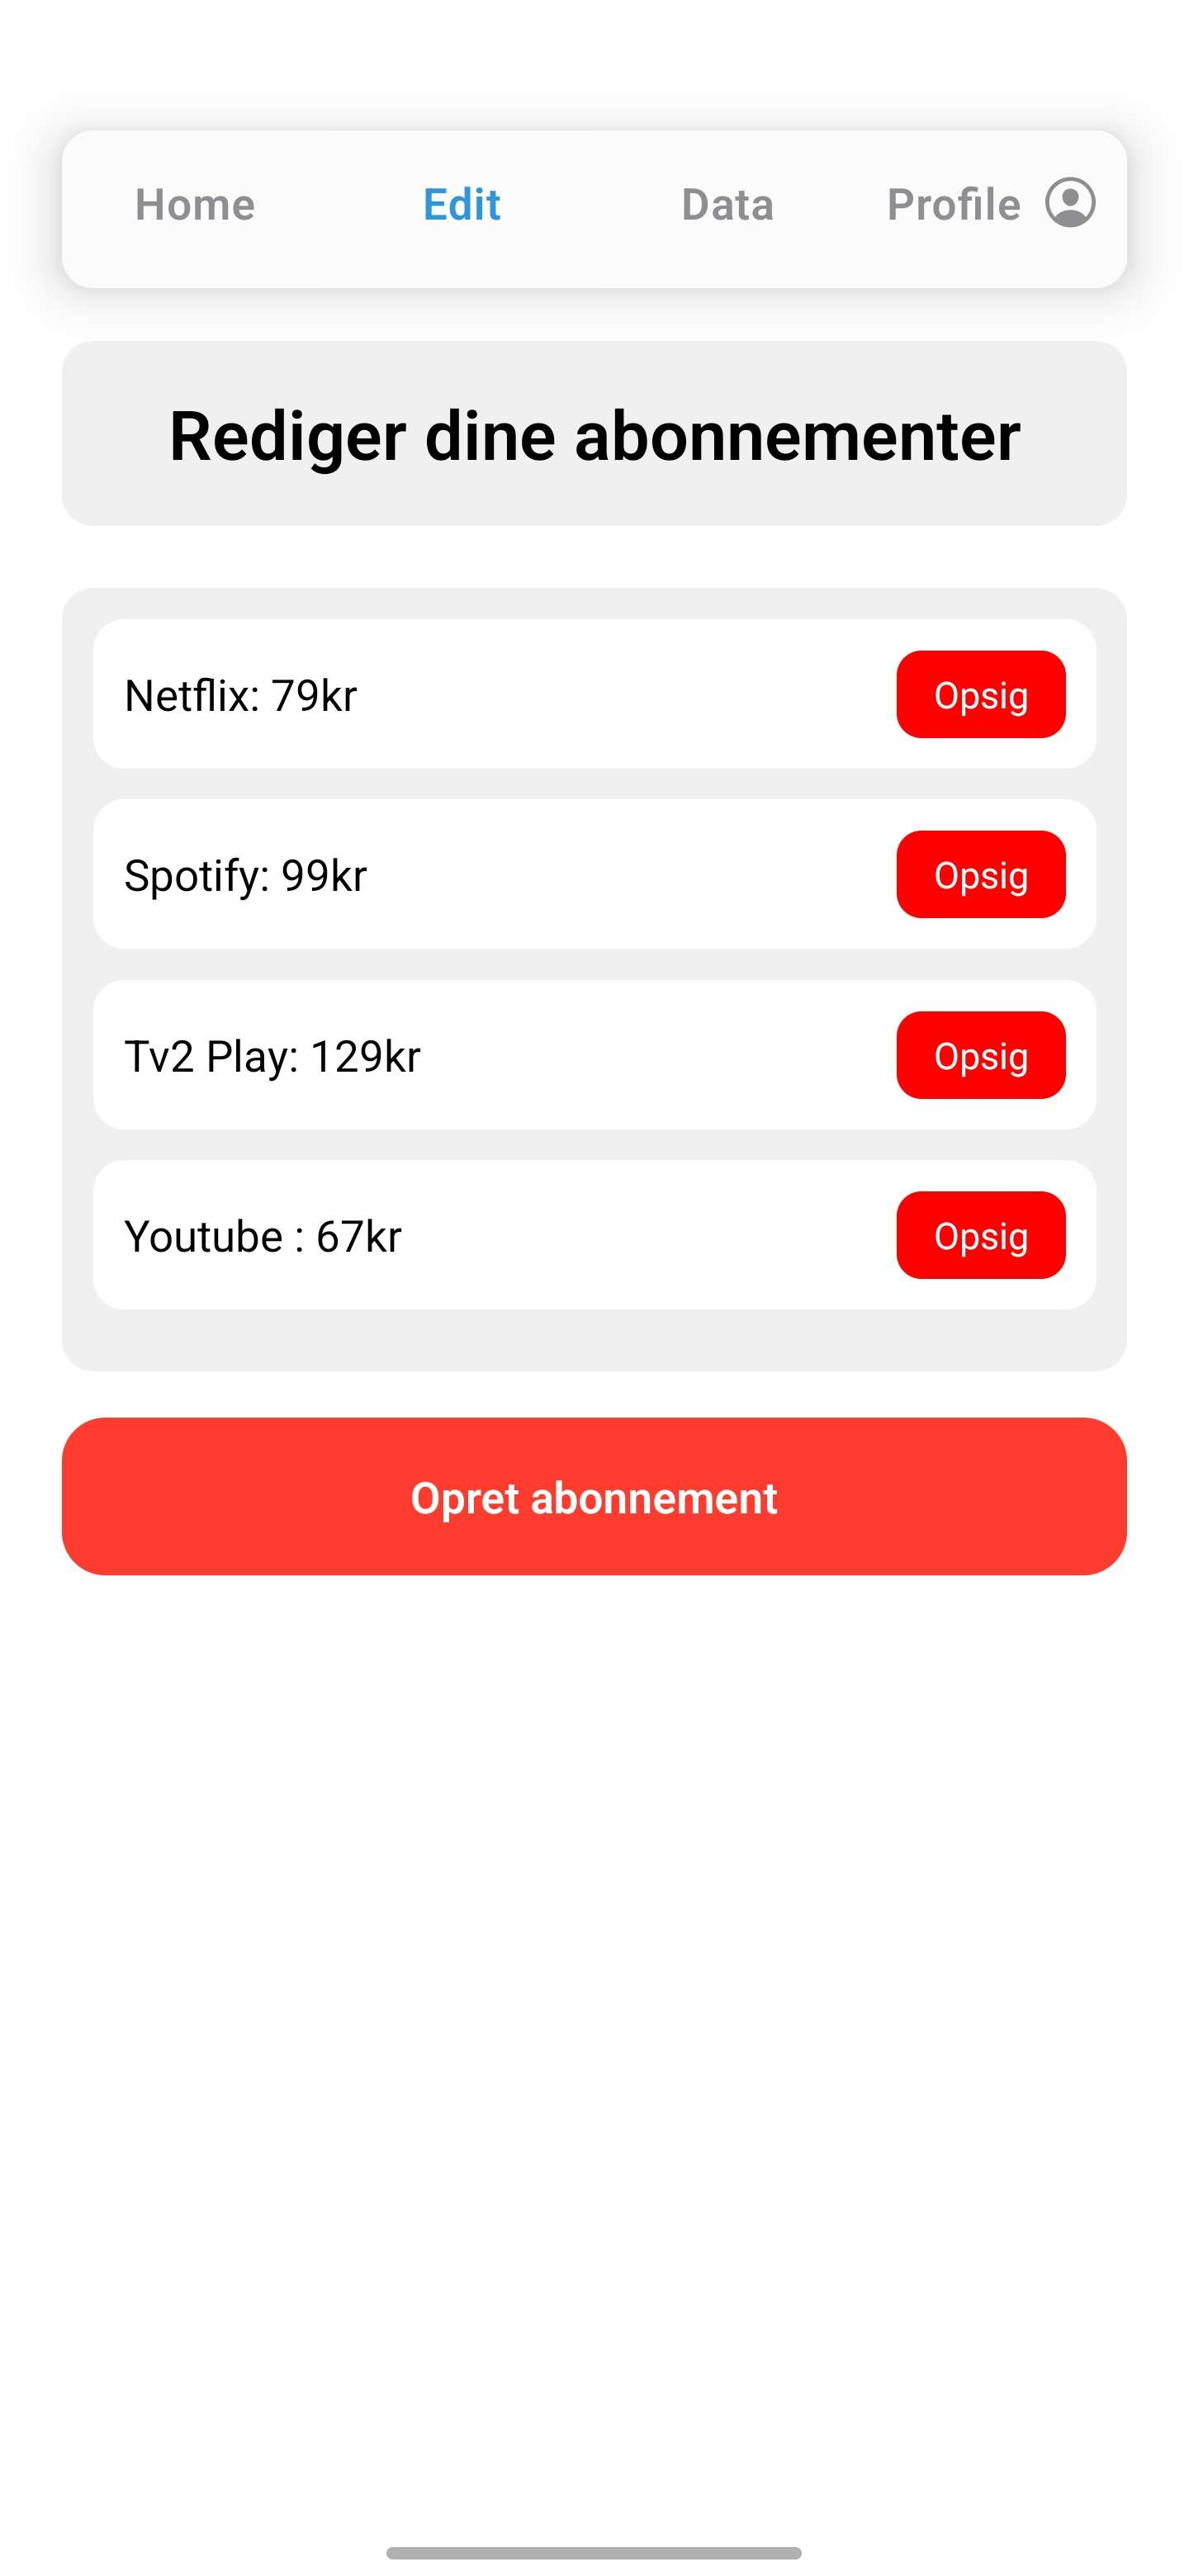
\includegraphics[width=0.5\textwidth]{assets/hifi-skitser/edit.jpg}}
  \end{figure}
\end{landscape}
\begin{landscape}
  \begin{figure}
    \fbox{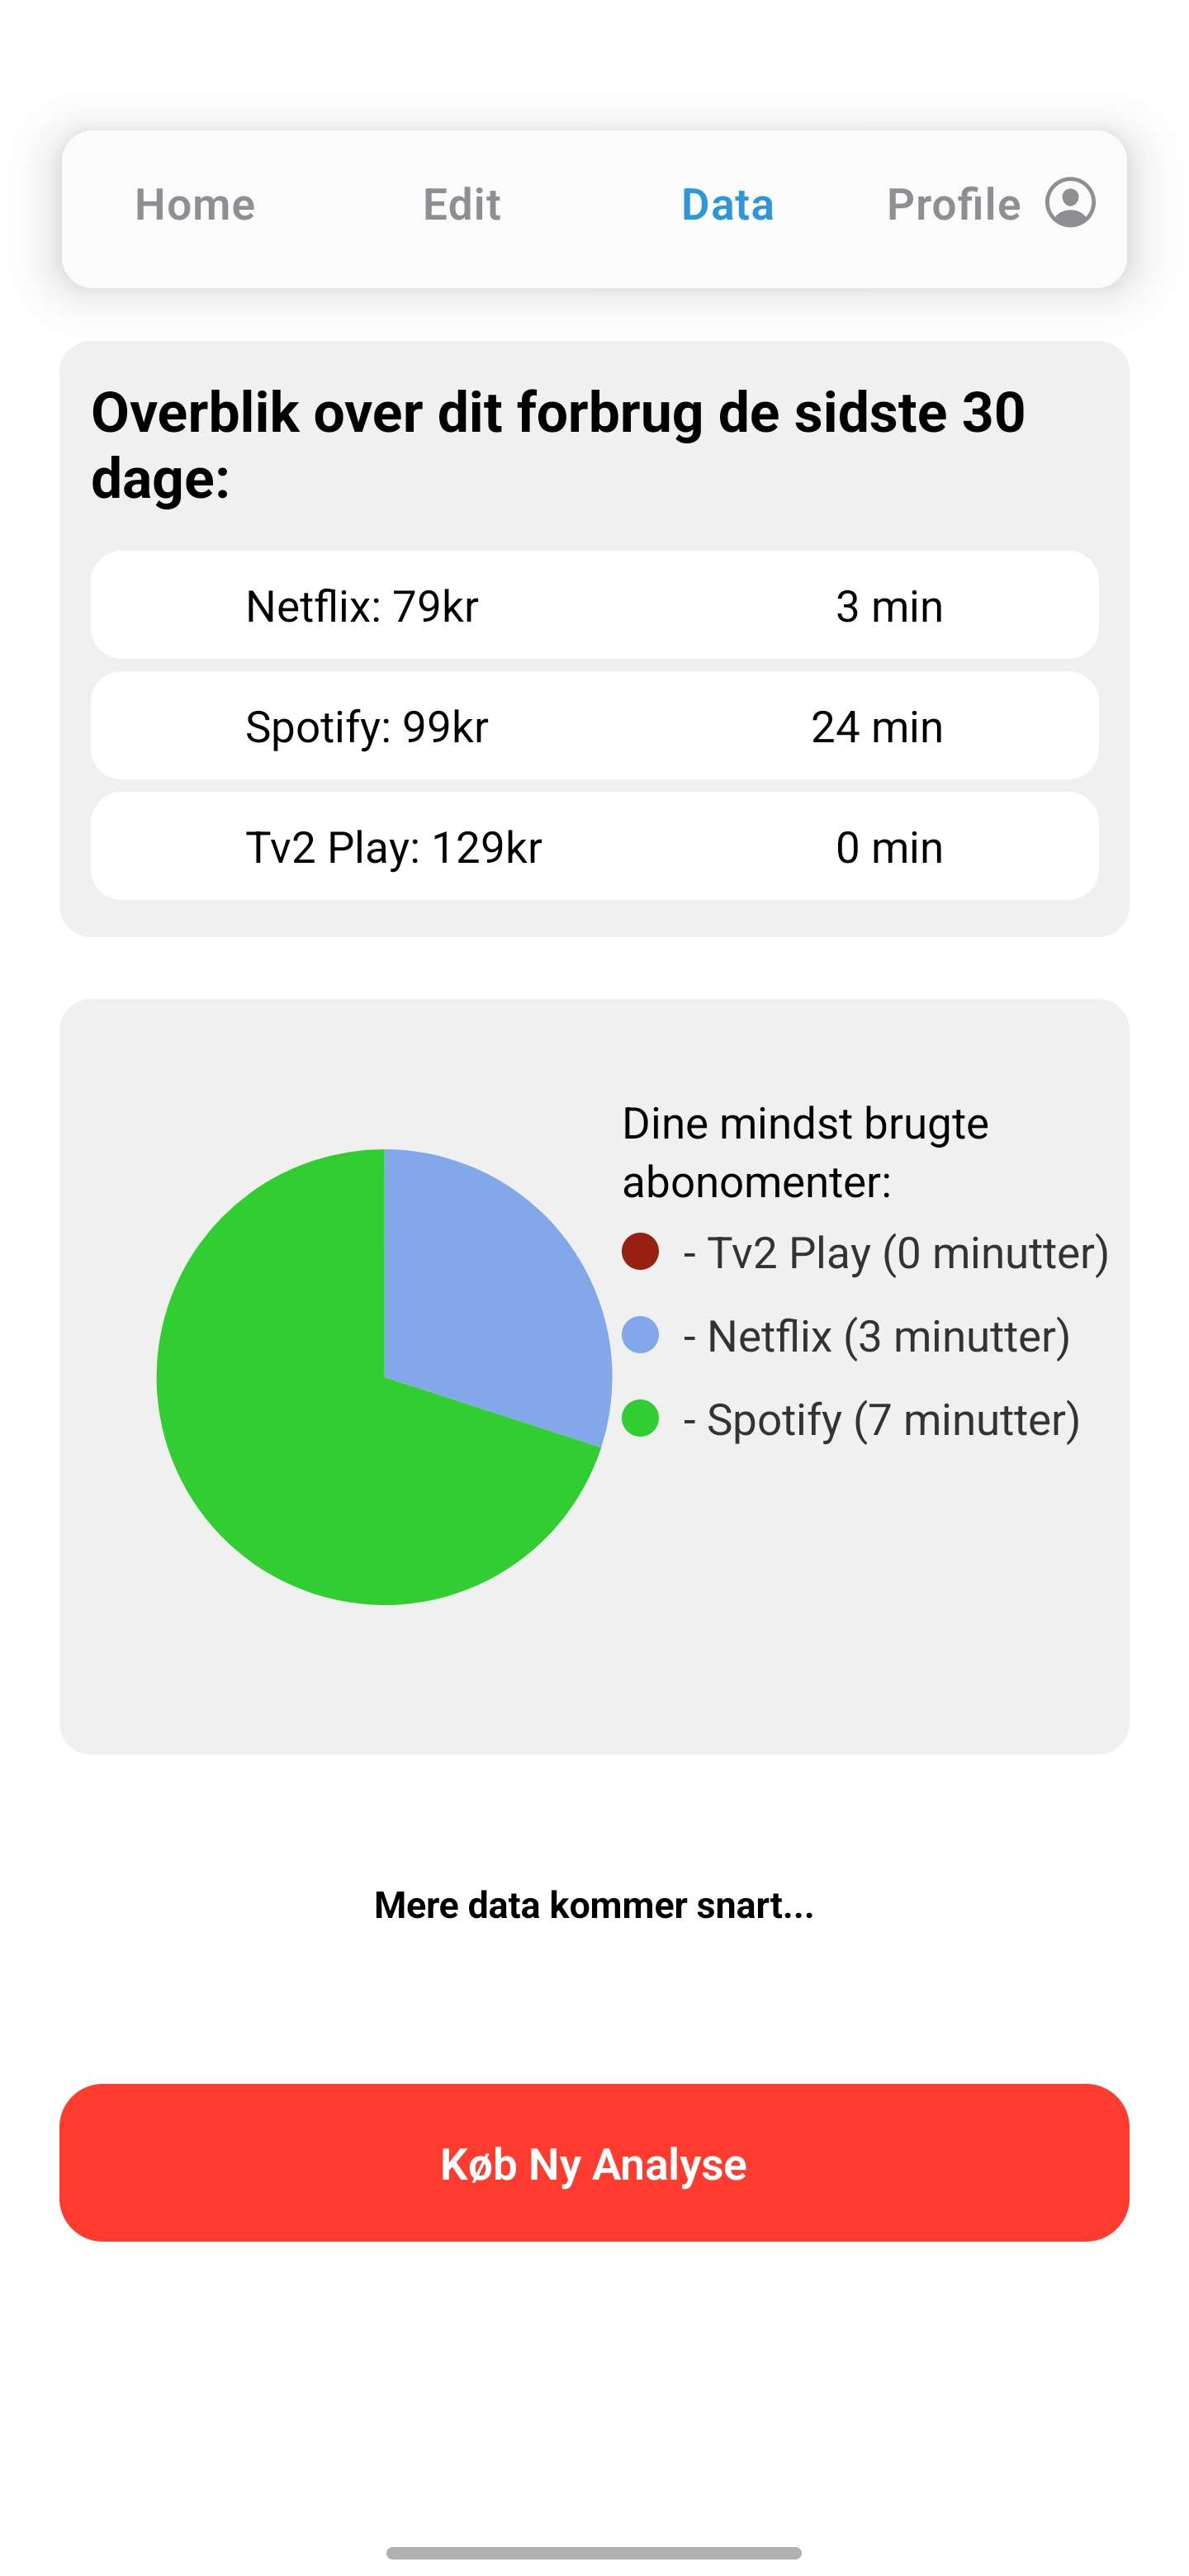
\includegraphics[width=0.5\textwidth]{assets/hifi-skitser/data.jpg}}
    \fbox{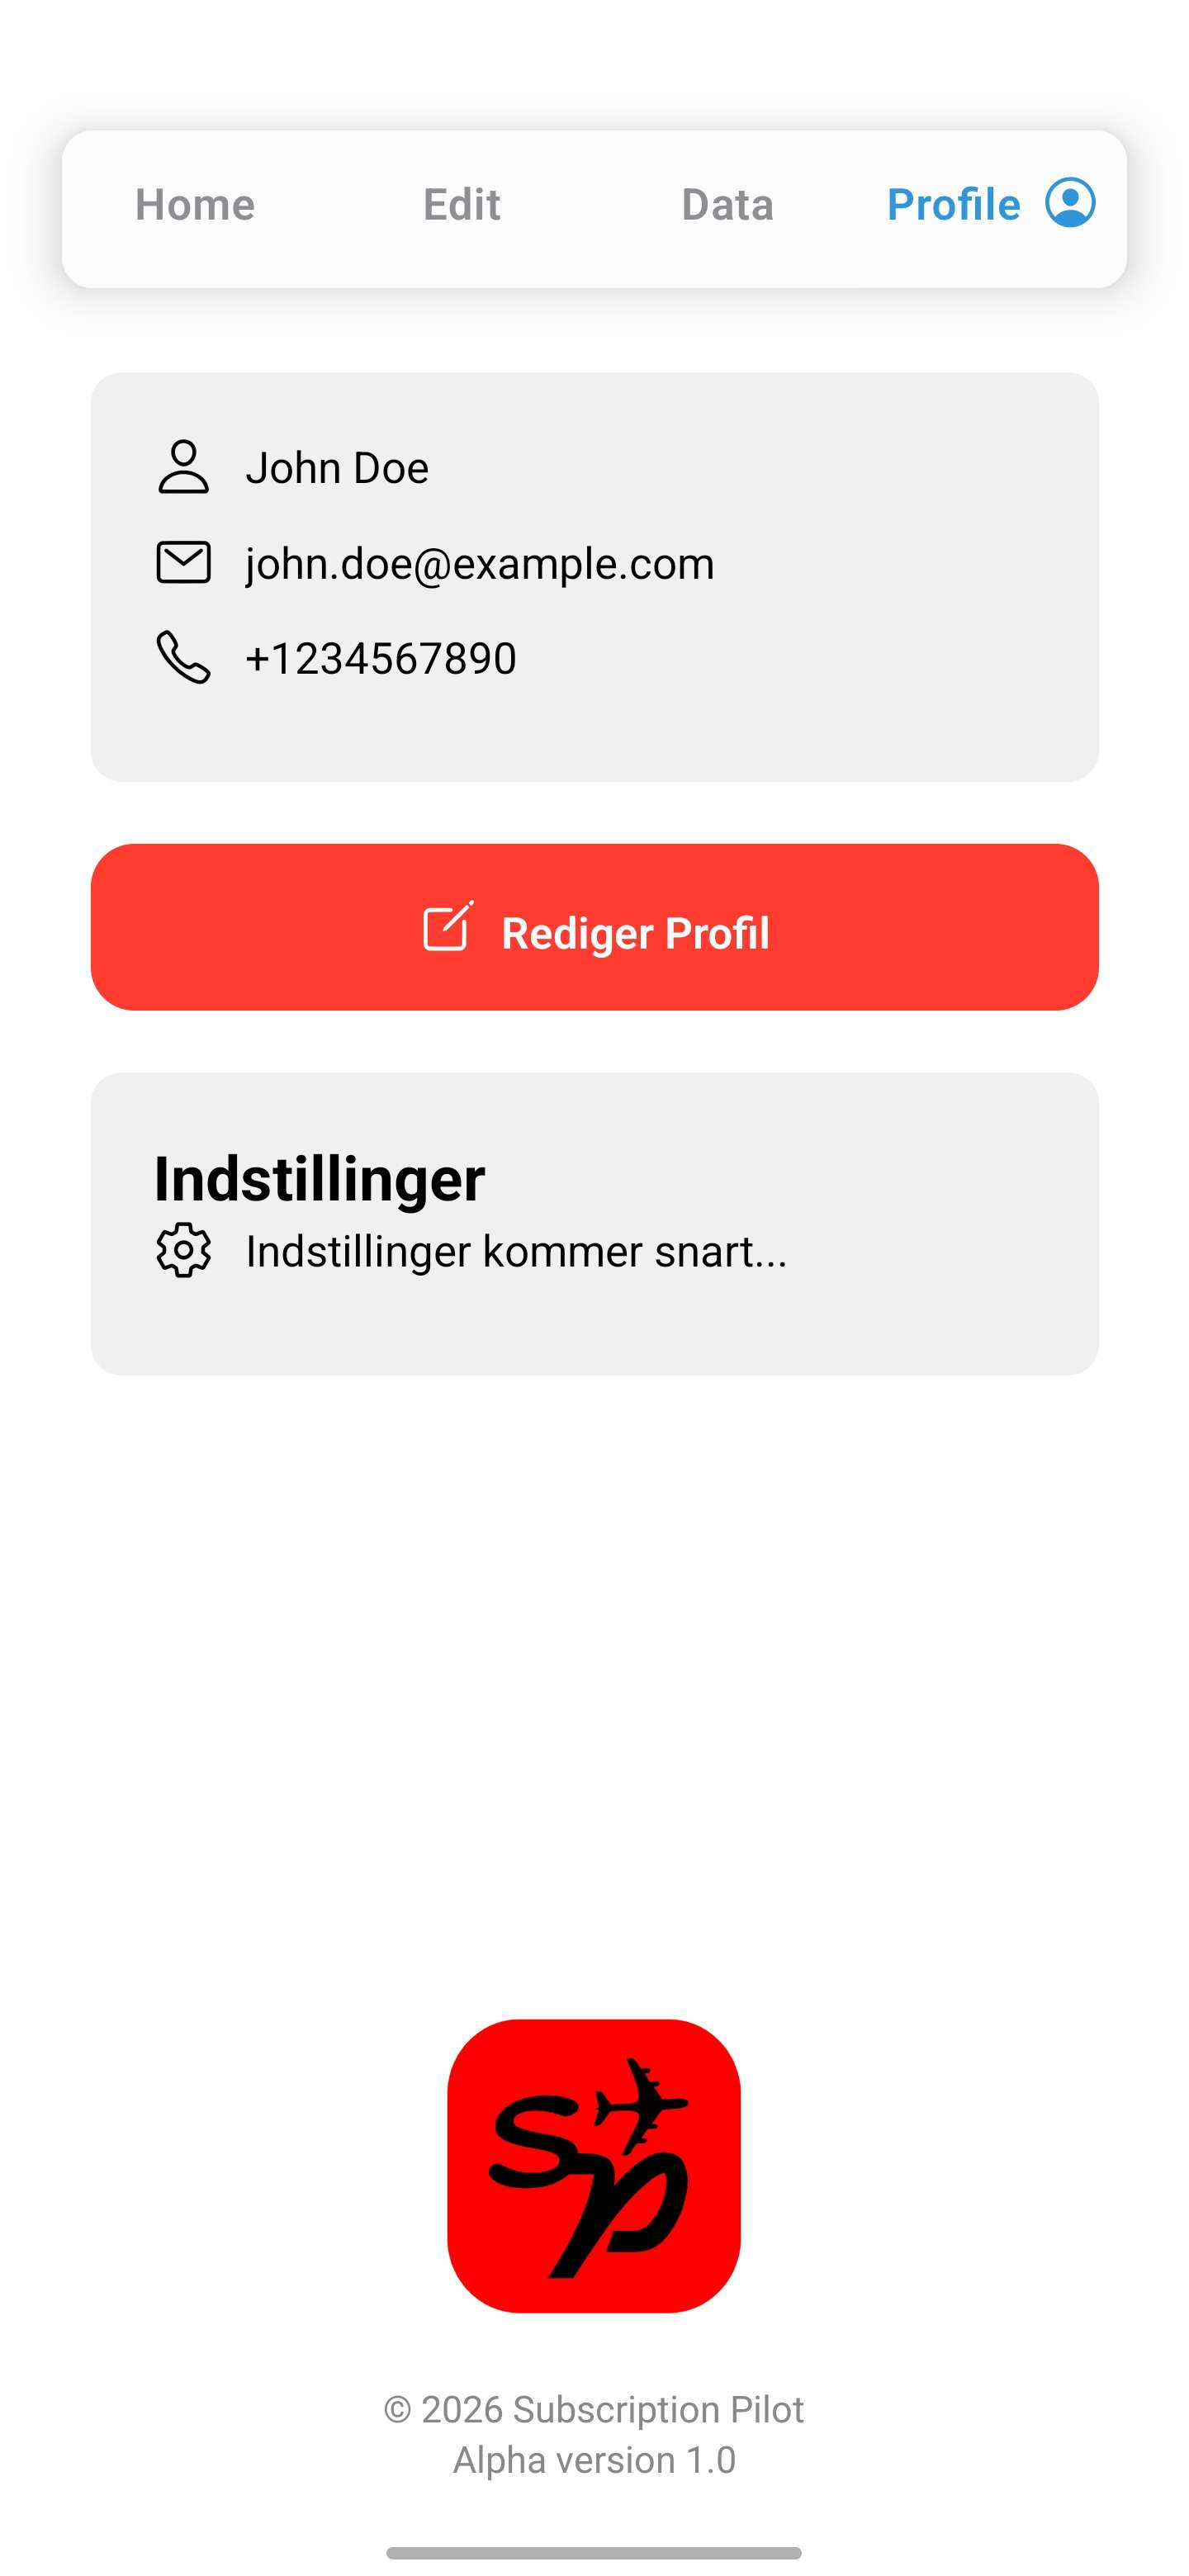
\includegraphics[width=0.5\textwidth]{assets/hifi-skitser/profile.jpg}}
  \end{figure}
\end{landscape}
    \end{appendices}
\end{document}
